\documentclass[11pt,a4paper]{report}
% Aberstwyth dissertation LaTeX Template
% Authors: Dr. Hannah Dee (hmd1@aber.ac.uk), Neil Taylor (nst@aber.ac.uk)
% This has been adapted from the Leeds Thesis template and the 
% Group Project template for Computer Science in Aberystywth University.
% 
% All comments and suggestions welcome.
%
% Template designed to be used with pdflatex: it may need alteration to
% run with a different LaTeX engine.
%
% Note - this is offered as a starting point for your work. You are not 
% required to use this template and can choose to create your own document 
% without it. 

% To build document on the unix command line, run four commands:
 
% pdflatex dissertation
% bibtex dissertation
% pdflatex dissertation
% pdflatex dissertation

% you will end up with dissertation.pdf 
\usepackage{mmp}

% the following packages are used for citations - You only need to include one. 
%
% Use the cite package if you are using the numeric style (e.g. IEEEannot). 
% Use the natbib package if you are using the author-date style (e.g. authordate2annot). 
% Only use one of these and comment out the other one. 
\usepackage{cite}
%\usepackage{natbib}

% Allow up to 4 levels of nesting of sub-sub sections
\setcounter{secnumdepth}{4}

% Use the following to selectively exclude chapters
%\includeonly{cover,abstract,acknowledge,declare,chapter1,chapter2}

\begin{document}

\captionsetup{justification=centering}

% all of the include directives below refer to tex files
% so \title{Aber Fitness Project}

% Your names
\author{Adam Lancaster [arl4], Andrew Edwards [ane18], Charlie Lathbury [ckl2], Daniel Monaghan [dkm2], David Fairbrother [daf5], Jack Thomson [jat36], James Britton [jhb15], Robert Mouncer [rdm10]}

\modulecode{SEM5640} % i.e. CS39440, CC39440, CS39620
\moduletitle{Developing Advanced Internet Based Applications} % i.e. Major Project or Minor Project

\date{\today} % i.e. the date of this version of the report

\status{Release} % Use draft until you create the release version. Then, change this to Release.
\version{1.0.1}

\maketitle



 includes cover.tex - to change the content,
% edit the tex file

\pagenumbering{roman}

% This is the front page
\title{Aber Fitness Project}

% Your names
\author{Adam Lancaster [arl4], Andrew Edwards [ane18], Charlie Lathbury [ckl2], Daniel Monaghan [dkm2], David Fairbrother [daf5], Jack Thomson [jat36], James Britton [jhb15], Robert Mouncer [rdm10]}

\modulecode{SEM5640} % i.e. CS39440, CC39440, CS39620
\moduletitle{Developing Advanced Internet Based Applications} % i.e. Major Project or Minor Project

\date{\today} % i.e. the date of this version of the report

\status{Release} % Use draft until you create the release version. Then, change this to Release.
\version{1.0.1}

\maketitle



               

\setlength{\textwidth}{7in}
\setlength{\oddsidemargin}{-0.4in} \setlength{\evensidemargin}{0in}         

% Set up page numbering
\pagestyle{empty}

% declarations of originality 
\textbf{Declaration of Originality: waiting on neil for this}               

\pagenumbering{roman}
\pagestyle{fancy}
\fancyhead{}
\fancyfoot[C]{\thepage}
\renewcommand{\headrulewidth}{0 pt}
\renewcommand{\chaptermark}[1]{\markboth{#1}{}}

\tableofcontents   
\newpage
\listoffigures
\newpage 

% Set up page numbering
\pagenumbering{arabic}

\setchapterheaderfooter

% include the chapters
\chapter{Overview}

\begin{center}
	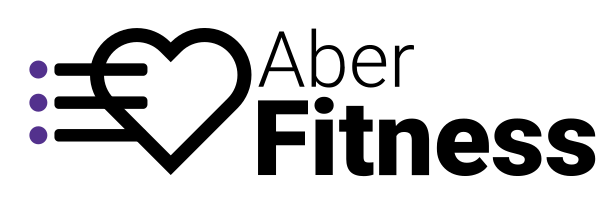
\includegraphics[width=0.5\textwidth]{Images/aberfitness.png}
\end{center}

\par
\textit{Aber Fitness} is a web application developed using Microsoft's \textit{.NET Core} and Oracle's \textit{Java Enterprise Edition} (henceforth referred to as Java EE). The project aims to provide a service which encourages fitness and promotes engagement with sporting activities amongst the users of the application, by offering functionality such as:

\begin{itemize}
	\item Graphing fitness data gathered by owners of \textit{Fitbit} devices, or through manual input.
	\item The ability to take part in challenges based on that fitness data.
	\item Providing a Sport ladder system, which has tight integration with a bespoke facility booking system.
\end{itemize}

\textit{Aber Fitness} aims to offer everything required by a sporty and active person in order to bring their sporting activities onto a digital platform and also to enhance their use of devices they already own, such as fitness tracking devices or smart watches such as the \textit{Fitbit Charge}.

\par
At launch, the system will automatically ingest activity data from \textit{Fitbit}, and be open to the addition of other health data provider services, such as Apple Watch, at a later date due to the modular nature of the data ingest system. Once normalised, this activity data will be used throughout the various microservices within \textit{Aber Fitness}, providing users with functionality such as a dashboard overview of their activity over the past month, as well as integrating tightly with the challenges microservice to add a competitive aspect to the system, with the aim of keeping users engaged with both the platform itself and keeping fit in general.

\par
\textit{Aber Fitness} will also feature a number of supporting tools, such as:

\begin{itemize}
	\item A user management system with two-factor authentication.
	\item A comprehensive audit trail of when and how their data was used and accessed, which is filterable by date.
	\item A global layout template with a dynamic sidebar, which can be adjusted by administrators. Those changes will be instantly propagated to the other microservices.
\end{itemize}

\par
\textit{Aber Fitness} is also designed to be scalable and easily deployed through the use of \textit{Docker}, by segregating related functionality into individual microservices.

\chapter{Requirements}

\section{Data Gathering and Storage}
\begin{tabular}{ |p{5cm}|l|l|p{8cm}|}
\hline
\textbf{Requirement}	&	\textbf{FR\#}	&	\textbf{Completed}	&	\textbf{Comments} \\
\hline
Management of Participants in the System			& DG-FR1	& Yes	& All sub requirements have been met. \\
\hline
Activity Data										& DG-FR2	& No	& Not all sub requirements have been met. \\
\hline
Linking a participant to a server-based data source	& DG-FR3	& Yes	& Requirement complete. \\
\hline
Obtaining data from the server-based data source	& DG-FR4	& Yes	& Requirement complete. \\
\hline
Receiving data from other devices					& DG-FR5	& Yes	& Requirement complete. \\
\hline
Receiving manual input of data						& DG-FR6	& Yes	& Requirement complete. \\
\hline
Data to retrieve 									& DG-FR7	& Yes	& Additional Requirement - All step data should be collected for the system. This will include "workout" sessions. \\
\hline
Removing data for a participant						& DG-FR8	& No	& TODO: May need changing. Not all sub requirements have been met. \\
\hline
Administrator access to data						& DG-FR9	& No	& Not all sub requirements have been met. \\
\hline
User group relationship								& DG-FR10	& Yes	& Additional Requirement - A user can exist on the system without being part of  a group. If a user joins a group they can only be associated with that one group. \\
\hline
Activity data management							& DG-FR11	& Yes	& Additional Requirement - An interface should be provided for the administrator to map FitBit activities to the activities created for the system. \\
\hline
\end{tabular}

\section{User Management}
\begin{tabular}{ |p{5cm}|l|l|p{8cm}|}
\hline
\textbf{Requirement}	&	\textbf{FR\#}	&	\textbf{Completed}	&	\textbf{Comments} \\
\hline
Authentication and authorisation 					& UM-FR1 	& Yes 		& Requirement Complete. \\
\hline
Local User Accounts 								& UM-FR2 	& Yes 		& Additional Requirement - The user accounts do not need to be Aberystwyth University integrated. Local user accounts should be used. \\
\hline
User Characteristics								& UM-FR3	& Yes		& Requirement specified in document but not given a functional requirement number. There will be three different types of users: member, coordinator and administrator. \\

\hline
\end{tabular}



\section{Health Dashboard}
\begin{tabular}{ |p{5cm}|l|l|p{8cm}|}
\hline
\textbf{Requirement}	&	\textbf{FR\#}	&	\textbf{Completed}	&	\textbf{Comments} \\
\hline
Review data for a member 							& HD-FR1 	& Yes 		& Requirement complete. \\
\hline
Set goals and view progress. 						& HD-FR2 	& Yes		& Requirement complete. \\

\hline
\end{tabular}


\section{Challenges}
\begin{tabular}{ |p{5cm}|l|l|p{8cm}|}
\hline
\textbf{Requirement}	&	\textbf{FR\#}	&	\textbf{Completed}	&	\textbf{Comments} \\
\hline
Create a challenge 									& C-FR1 	& Yes 		& Requirement Complete. \\
\hline
Join a challenge 									& C-FR2 	& Yes  		& Requirement Complete. \\
\hline
Activity during a challenge							& C-FR3 	& Yes 		& Requirement Complete. \\
\hline
Closing the challenge								& C-FR4		& Yes 		& Requirement Complete. \\
\hline
Types of challenges 								& C-FR5 	& Yes		& Additional requirement - There should be two types of challenge. "Personal goals" which will be individual challenges and "Group challenges" which allows members to join challenges for their group. \\

\hline
\end{tabular}


\section{Booking System}
\begin{tabular}{ |p{5cm}|l|l|p{8cm}|}
\hline
\textbf{Requirement}	&	\textbf{FR\#}	&	\textbf{Completed}	&	\textbf{Comments} \\
\hline
Facilities      									& BS-FR1	& Yes      		& Requirement complete. \\
\hline
Availability   										& BS-FR2	& Yes      		& Requirement complete. Requirement extended - an administrator block on a facility should be a single booking not multiple hourly bookings. 	\\
\hline
Booking         									& BS-FR3	& Yes      		& Requirement complete. \\
\hline
Available Times 									& BS-FR4	& Yes      		& Additional Requirement - A fixed time for bookings should be available for a facility (9am -9pm). \\

\hline
\end{tabular}

\section{Sports Ladder}
\begin{tabular}{ |p{5cm}|l|l|p{8cm}|}
\hline
\textbf{Requirement}	&	\textbf{FR\#}	&	\textbf{Completed}	&	\textbf{Comments} \\
\hline
Creating 											& SL-FR1	& Yes 		& Requirement complete. \\
\hline
Joining 											& SL-FR2	& Yes 		& Requirement complete. \\
\hline
Profile Update 										& SL-FR3	& Yes		& Requirement complete. \\
\hline
Suspension 											& SL-FR4	& Yes 		& Requirement complete. \\
\hline
Current Ladder	 									& SL-FR5	& Yes 		& Requirement complete. \\
\hline
View Member											& SL-FR6	& Yes 		& Requirement complete. \\
\hline
Challenge 											& SL-FR7	& Yes		& Requirement complete. \\
\hline
Scheduling 											& SL-FR8	& Yes 		& Requirement complete. \\
\hline
Response to a challenge 							& SL-FR9 	& Yes 		& Requirement complete. \\
\hline
Expiry 												& SL-FR10 	& Yes		& Requirement complete. \\
\hline
Result 												& SL-FR11 	& Yes 		& Requirement complete. \\
\hline
Removal 											& SL-FR12 	& Yes 		& Requirement complete. \\
\hline
Match Involvement									& SL-FR13 	& Yes 		& Additional Requirement - As a member can only be involved in one match at a time. \\
\hline
Winning a match 									& SL-FR14 	& Yes 		& Additional Requirement - If the loser of a match is in a high position on the ladder than the loser, their position should swap with the loser on the ladder. \\

\hline
\end{tabular}

\section{Engagement}
\begin{tabular}{ |p{5cm}|l|l|p{8cm}|}
\hline
\textbf{Requirement}	&	\textbf{FR\#}	&	\textbf{Completed}	&	\textbf{Comments} \\
\hline
Current Rankings 									& E-FR1		& Yes	& Requirement complete. \\
\hline
Individual Progress									& E-FR2		& Yes	& Requirement complete. \\
\hline
Weekly Updates 										& E-FR3		& Yes	& Requirement complete. \\
\hline
Missing Reading Updates 							& E-FR4		& Yes	& Requirement complete. \\

\hline
\end{tabular}


\section{External Interface}
\begin{tabular}{ |p{5cm}|l|l|p{8cm}|}
\hline
\textbf{Requirement}	&	\textbf{FR\#}	&	\textbf{Completed}	&	\textbf{Comments} \\
\hline
Appearance & EIR1 & Yes. & Requirement Complete. \\
\hline
Internationalised Interface & EIR2 & No. & Requirement not complete. \\
\hline
Handling UI - Proxy & EIR3 & Yes. & Additional Requirement - Services should generate their own UI, the UI goes back to the client via a proxy. \\
\hline
\end{tabular}
\chapter{Development Methodolgy}

\textcolor{red}{\textbf{TODO: Possibly restructure this, it\'s a start for now. Not 100\% sure what Neil\'s looking for here.}}

Upon starting the project, we met as a group and decided on a standard style of development which would work best between all of us. After some discussion, we concluded that a \textit{Scrumban}\cite{scrumban} style of development would best fit our needs. Due to the relatively short duration of the project, and our team consisting of only eight developers, we decided on adopting this rather hands off development approach which focuses on flexibility and being able to change and adapt the project plan and sprints as the project progresses. The \textit{Scrumban} methodology was also suited to the project as the two technologies we were required to use, Java EE and .NET Core, were new to all of the members of our team, making estimating sprints and velocity quite difficult. 

We began the project by breaking the project specification down into disitinct microservices, and deciding which technologies would be best suited to each service. \textbf{TODO: Link to figure below}

\begin{figure}[H]
    \centering
    \includegraphics[width=\textwidth]{Images/Initial_Spec_Chart.jpg}
    \caption{An initial design diagram which was used to help break down the project into smaller microservices and gain a rough understanding how each microservice could interact}
\end{figure}

Once the individual microservices had been decided upon, we set out on allocating each microservice to two members of the team and assinging each service a priority ranking between 1 and 3, depending on how the services depended on one another. Services marked with a priority of 1 were core parts of the \textit{AberFitness} infrastructure on which many other parts of the system relied on their APIs in order to function correctly, such as the \textit{Health Data Repository} microservice.  \textbf{TODO: Link to figure below}

\begin{figure}[H]
    \centering
    \includegraphics[width=\textwidth]{Images/Numbering_Microservices.jpg}
    \caption{Initial plan for ordering microservices in terms of priority and allocating them to members of the team for development}
\end{figure}
\chapter{Design}

\section{System Overview}
The \textit{Aber Fitness} system is broken down into a number of microservices in order to aid portability, scalability and promotes a more maintainable codebase. After reviewing the initial project specification, the following microservices were created:

\begin{itemize}

	\item \textbf{Booking \& Facilities} - The \textit{Aber Fitness} offers functionality for users to be able to schedule bookings at sports venues, such as swimming pools and squash courts. This microservice is called used by the \textit{Ladders} service to create bookings for competitions.

	\item \textbf{Challenges} - The system offers the ability to give users activity challenges, for example completing a number of steps in a specific timeframe. These challenges can also be 'group' challenges, where a number of users can compete against each another to achieve goals such as furthest distance walked in a week, etc.

	\item \textbf{Communications} - This microservice provides an API for other services to send email notifications to users. It does not present any form of web UI, and users do not directly interact with it. This system could also be easily expanded to send out text messages, push alerts, etc. depending on future requirements.

	\item \textbf{Fitbit Ingest Service} - At launch, the \textit{Aber Fitness} platform allows a user to link their \textit{Fitbit} accounts to the system in order to import their activity data. The service periodically polls the Fitbit API for new data on the users' behalf, then stores this into the \textit{Health Data Repository}.
	
	\par With the possibility of adding future platform support the "ingest service" concept was created. This would allow us to support services such as Apple's \textit{HealthKit} and other fitness tech providers. 
	This architectural design means that activity data can be normalised by a number of "ingest services" before being passed through to the \textit{Health Data Repository} service for storage. 

	\item \textbf{Gatekeeper} - \textit{Gatekeeper} is \textit{Aber Fitness}'s OpenID Provider, and handles all authentication within the system. User credentials and account metadata is stored within \textit{Gatekeeper}\textit{Gatekeeper} uses the OAuth 2.0 flow and is responsible for providing a single sign-on service for all of the various microservices. Microservices also contact \textit{Gatekeeper} to obtain and verify tokens when calling internal APIs.

	\item \textbf{GLaDOS} - \textit{GLaDOS} is the centralised auditing mechanism for \textit{Aber Fitness}. It presents a REST API which is used to store audit data; such as when a user's data was accessed, modified, or deleted. \textit{GLaDOS} also provides a Status page which displays the availability of all the other microservices.

	\item \textbf{Health Dashboard} - \textit{Health Dashboard} is the first interface users will encounter after logging in, or navigating to \textit{Aber Fitness}.  It provides the user with an overview of their recent activity as well as providing updates on any challenges or ladder competitions the user may be involved in.

	\item \textbf{Health Data Repository} - The \textit{Health Data Repository} service is responsible for providing an API for accessing and storing activity data. It receives normalised activity data from the Ingest Services, and provides multiple API endpoints for other microservices to access user activity data. 

	\item \textbf{Ladders} - \textit{Ladders} is responsible for organising and managing ladder style competitions among users of the system. Users can compete in sporting championships for a variety of competitive sports such as tennis, running or cycling etc. The \textit{Ladders} service also automatically books venues for upcoming competitive events, which is managed by the \textit{Booking Facilities} microservice.

	\item \textbf{User Groups} - \textit{Challenges} can also be turned into a competition amongst users of a group. For example, a group may consist of a few friends or an entire office department. Users within a group compete to complete goals, such as who can achieve the most steps in a single day. The \textit{User Groups} service is responsible for managing users into groups, and allowing users to leave and join other groups.

\end{itemize}
\chapter{Implementation}

\section{Deployment}

\section{Java EE}
    \subsection{Common Components}
        \subsubsection{Handling Dependencies and Static Analysis}
        \par
        At the start of the project the JavaEE development teams agreed to use \textit{Maven}\cite{Maven} to handle their dependencies. This allows the entire build process to be ran at the commandline rather than within the IDE, which is essential for \textit{TravisCI} integration.

        \par
        Maven uses an XML file called \textit{POM.xml} to define the dependency names, versions and additional options. These are fetched from Maven Central and cached locally for future builds. To add a new dependency a developer simply visits the hosting website and copies the XML provided alongside each package. Additionally developers can use the \textit{Scope} option which instructs the packaging plugin the associated \textit{JAR} files are provided by the Payara runtime.
        
        \par
        \textit{IntelliJ} natively supports reading from Maven's \textit{POM.xml} file, which defines the list of dependencies and compilation steps. Maven also contains a plugin which allows developers to package the built files into a web archive (WAR). This did have some caveats however; running 
        `\textit{mvn war:war}' would result packaging artefacts from the previous compilation, without compiling the current application. This could lead to confusion as new changes would no be reflected without `\textit{mvn compile war:war}'.

        \par
        Whilst working locally developers could still rely on IntelliJ's built in mechanism for packaging and deploying to a local Payara instance. This allowed for rapid development feedback and iteration without the overhead imposed by Maven.

        \subsubsection{Creating Docker Images}
        \par
        By utilising the ability to run the entire build process on the command-line with Maven we were able to quickly add Travis CI integration. This would clean compile the entire application, run the full \textit{JUnit} test suite and lastly package a WAR file.

        \par
        Initially we used \textit{CheckStyle} to also enforce coding style conventions. However the rules were over-specified. Additionally, unlike other formatting tools there was no option to emit a patch-file which allows developers to automatically fix-up many errors such as incorrect white space or formatting.

        \par
        The Java teams migrated to the \textit{PMD}\cite{PMD} static analysis tool: this warns about unused fields and variables, unsafe constructs,and dangerous coding patterns.
        The Maven test target was modified to run the \textit{PMD}\cite{PMD} static analysis tool before any unit tests. If any violations were detected the build would immediately stop, ensuring all modifications were inspected.

        \par
        The groups proceeded to add a \textit{Dockerfile} to build a docker image for later deployment. Payara provide multiple images on \textit{DockerHub}\cite{DockerHub_Payara}, which range from the full server to an embedded instance.

        \par
        Initially we copied the local web archive, which was built on Travis, into the full Payara deployment folder. This allowed us to use the web administration console to resolve various deployment issues without having to dig through log files. After moving changing the default source code layout, which resolved \textit{resources} not being included in the final archive, we successfully deployed GLaDOS to the full instance.

        \par
        However we could not get Fitbit Ingest to successfully deploy, they had already started implementing the OAuth flow which is required by both the Fitbit API and our own internal API. The internal SSL implementation had changed with JDK update 191, which prevented the \textit{CDI} layer from initialising the associated beans.

        \par
        As the bundled JDK version is controlled by Payara in the base image we proceeded to look for an alternative solution. We decided against modifying the image to transplant a specific JDK at build time. Instead, we found that there was an open upstream issue\cite{payara_ssl_issue} that used reflection to resolve the problem internally. As this fix was not released into the latest stable release we had to switch to running pre-release images for all Java EE applications.

        \subsubsection{Migrating to Micro Image}
        \par
        The Payara Microprofile image is designed specifically to be used in Docker deployments. Whilst this does not implement the full EE, the memory usage is ten times lower at 90MB. The profile still provided the required set of services for the application so there was a significant benefit to completing this migration. However trying to deploy to the micro instance resulted in an exception being thrown whilst completing the implicit bean discovery phase. 

        \par
        The CDI 1.1 specification and above requires the server to automatically scan for injection points and pair it with matching enterprise Java beans (EJBs). This can fail with older dependencies, so we initially suspected one of the dependencies did not correctly use the \textit{beans.xml} annotation to turn this off.
        \newline
        Switching off bean discovery and manually annotating them allowed the ingest service to correctly deploy. However bean discovery is required for Facelets 4.0 and an exception will be thrown if it is not enabled. A new project was created with all but the essential dependencies removed, and we discovered the exception was still thrown which only added to the confusion. 
        
        \par
        By looking at the package namespaces associated with the injection points and running `mvn dependency:tree' we could see that `\textit{org.sonatype.guice}' was the culprit. Walking up the tree we discovered that the WAR plugin was being included in our packaged dependencies. At deployment the microprofile server tried to start a Maven instance and failed, thus removing this dependency correctly allowed the application to start. The development teams realised that the plugin was included in our installed copies so we could still continue to use it.

        \label{JTA_Targets}
        \subsubsection{Setting up JTA Targets}
        Both services started off by instantiating the single JDBC connection through the driver manager as required. This had some caveats however: Firstly, the JDBC driver had to be distributed and managed within the web archive. Secondly, there was no form of connection pooling to allow for scaling at the persistence layer.

        \par
        Traditionally a connection pool is created using the administration web GUI. However this would require a developer set up the pool each time continuous deployment finished on a full instance. The microprofile we had just switched to did not provide a web GUI at all.

        \par
        Glassfish allows a web application to specify resources found on the server using `glassfish-resources.xml'. This XML file can also use system environment variables allowing us to protect and specify database credentials on the deployment targets. The examples found online primarily pertained to a \textit{MySQL} deployment, so multiple iterations of testing and deployment were required to get the pool working successfully. This switch allows an application to detect and create connection pools at deployment, allowing the images to rapidly redeploy facing another database instance.

    \subsection{Fitbit Ingest Service}
        \subsubsection{To Do}

    \subsection{GLaDOS}
        \subsubsection{REST API}
        \par
        The primary role of GLaDOS is to store audit data so that users can view how their data was viewed and modified. Whilst there are native implementations, such as the Java Messaging Service, these require the calls be proxied into a local JVM instance to handle the transport component. We chose to serialise into JSON and use REST as the transport mechanism as all applications had native support for this set up.

        \par
        \textit{JAX-RS} is an API specification for JSON parsing in Java, additionally Payara provides \textit{Jersey} as the implementation of this API at runtime. This avoided us having to package additional dependencies into the web archive. This also allows us to build standard response pages based on the error code internally generated, avoiding having to develop error views.        

        \subsubsection{Unit Testing and Mocks}
        \par
        A new class abstracting the database layer allowed us to avoid writing entity handling at this. We instead focused on writing unit tests which verified the various endpoints correctly serialised or de-serialised data. \textit{Mockito}\cite{Mockito} allows developers to inject mock objects by specifying the class which the test fixture is using.

        \par
        We could not use dependency injection within the endpoint implementation, as the instantiation point is internal to the framework. This doesn't prevent us from using mocks as Mockito allows a developer to inject them through the reflection methods built into the library. A database call such as `\textit{db.getEntry(id)}' could be tested to see which status codes would be sent and verify the data,if any, was serialised correctly.

        \subsubsection{Integration Testing with Arquillian}
        \textit{Arquillian}\cite{Arquillian} allows developers to specify the classes to archive and deploy within the text fixture. Payara also provides an embedded Arquillian test container which can be ran at test time to exercise sections of a full system. This would allow us to write integration tests for an end-to-end operations, such as POSTing data to an endpoint and ensuring it is written to the persistence layer.

        \par
        There was extensive documentation on the methods required to pack an archive, but limited examples on handling Maven dependencies. As the embedded instance provides no runtime methods we were having problems getting the container to correctly run. Developers could specify the full class paths for their dependencies to ensure the were packaged, but this was extremely verbose and fragile.

        \par
        We looked into using the Maven dependency resolver, which allows developers to get a list of runtime Jars and package them into the archive. However this would led to another set of problems where Maven was trying to export them into a \textit{.zip} format, then throw an exception because this was not supported.

        \par
        With no easy was to control the format that runtime dependencies were exported in, combined with a lack of documentation pertaining specifically to Maven we agreed to abandon this method of automated testing. This would give us more time for implementing other components within the deadline. We opted to rely on manual integration testing for the duration of the project instead.

        \subsubsection{Entity Management}
        This service only persists Audit Data, therefore we ultimately need to persist a single entity. Whilst many ORM solutions exists for Java, such as \textit{Hibernate}, we decided against them due to the implementation overhead that was required.

        \par
        Instead we relied on the persistence layer provided in the EE specification. Using the connection pools which were set up for both Java services (see \ref{JTA_Targets}), we could specify which JTA the injected entity manager should use.

        \par
        The table schema is managed through annotations on an entity class. This also allows the implementation provided by Payara, \textit{EclipseLink}, to create the tables required at deployment time. As the framework relies on the field types to determine which underlying storage to use there is a hidden pitfall. If the type does not have a native serialisation Java will try to persist this using binary data.

        \par
        Instants are used to specify timestamps on logs, these are cross compatible as they use \textit{ISO 8601}\cite{ISO_8601}, a string specifier for absolute time points. This format allows both .NET Core and Java application to send timestamps in the following format \textit{2018-11-28T12:04:14Z}. However as this type was added in JDK 8 there is no native storage conversion built into the entity framework.

        \par
        Two adaptors were written based on the \textit{AttributeConverter} interface. These provide methods for marshalling and un-marshalling Instants into String objects, which the entity manager can easily store. Annotating the field installed the converting class and correctly updated the schema. This also has the added benefit of making the stored timestamps human readable within the database, which extremely helpful for debugging.

        \subsubsection{Developing Facelets}
        \par
        GLaDOS also provides a page that allows a user to retrieve audit data associated with their account. Administrators can look up any users audit data by user their unique ID too. In addition there is a status page which allows anyone to view the status of all other micro-services without logging in.

        \par
        The front-end of GLaDOS use facelets to implement the MVC pattern. A backing bean for the user data uses named queries from the persistence layer to retrieve data into a list of entity objects. We switched to using \textit{PrimeFaces}\cite{Primefaces}, which is a fork of the now deprecated \textit{RichFaces}. This allows us to use components such as \textit{DataTables} which dynamically generate tables based on the number of entries returned.

        \par
        The Fitbit Ingest Service had completed OAuth implementation for connecting to internal and external APIs. This was ported across to GLaDOS and further modified. As the ingest service has no front-end they don't need to persist \textit{JSON Web Tokens (JWTs)}. Additional methods were written specifically for this microservice. These include using the HTTP session handling built into the web framework to persist the token on the server. Another helper class was written which validates the stored JWT as the user navigates through protected pages, or POSTs any requests.

        \par
        Service statuses were implemented using a singleton Java bean which is instantiated at deployment. Using the scheduling capability provided for EJBs we poll all services every 20 seconds in a seperate thread. All services implement an endpoint at \textit{/api/status} that returns a 200 or 204. This is stored until the page is retrieved where the backing bean, acting as a presenter forward the results on.

        \par
        As the application stack uses an \textit{nginx} instance to reverse proxy queries the URLs must take this into account when they are generated within the facelet. .NET Core makes this trivial by calling `\textit{App.UsePathBase(URL)}' at start up, however Java applications rely on the context root. This was interfering with the URL rewriting that Nginx performs resulting in the service using the 
        `\textit{/glados/glados/}' base path.

        \par
        Initially we used an environment variable to manually generate links between the pages of the service and set the context root to 
        `\textit{/}'. However, this quickly proved to be untenable when using forms, as POST requests were being sent to 
        `\textit{/destination}' 
        rather than 
        `\textit{/glados/destination}'. Ultimately to work around this an exception was added to Nginx configuration to avoid re-writing any URLs for GLaDOS, and instead rely on the service to correctly address all requests. This allowed us to switch back to generating addresses based on the \textit{outcome} tag and use forms on the service.



\section{.NET Core}
    \subsection{}{Common Components}
some blurb about .net core here

    \subsection{Booking Facilities}

    \subsection{Challenges}

    \subsection{Communications}

    \subsection{Gatekeeper}

    \subsection{Health Data Repository}

    \subsection{Health Dashboard}

    \subsection{Ladders}

    \subsection{User Groups}

\chapter{Testing}
\par
One of the core tenets of continuous deployment is the reliance on a mix of automated and manual testing to ensure a system is functioning correctly. The applicable subset of these tests were run before each change specified in a pull request was accepted. The full suite is run as part of the release process, allowing developers to deploy the application to production with confidence.

- XUnit - recommended and widely used, Moq
- Moq - Gatekeeper
- JUnit
- Mockito - GLaDOS / Ingest (to fix)


\section{Integration Testing}
\par
Most of the micro-services provide internal APIs, which are not designed for external usage. To protect these endpoints the OAuth 2.0 flow was used to authorize application interactions with client credentials. Whilst unit testing ensures each API correctly responds according to its documented behaviour, it does not exercise all components that partake in an interaction.

\par
As REST endpoints were used as the primary message exchange method we could send and request JSON payloads to ensure the system under test behaved as expected. Multiple third party solutions were used for testing APIs, \textit{Postman}\cite{Postman} was one instance that was widely used by the development team. 
This can handle the OAuth flow 

\par
Developers used these tools to ensure that malformed requests or interaction with no authorization token were correctly handled. Additionally they can handle the OAuth flow on a developers behalf, this was extremely useful when debugging interactions between applications and resolving digressions from the API specifications.


\section{System Testing}
\par
Aber Fitness is deployed onto two separate docker hosts that represent staging and production. Developers trigger a deployment from the latest development images in Slack then manually test the system in a deployed state. This also allows us to detect deployment specific problems, which are un-testable without a complete system.

\par
One example of an issue caught by manual system testing was a controller which was not asynchronous. Unit tests would not exercise the instance in parallel, so this was not noticed through unit testing. When API calls were made to the deployed application a HTTP 502 was thrown. The controller was blocked on the original call and could not respond to the next call.


\section{Static Analysis}
\subsection{PMD}
\par
Initially, Java used \textit{CheckStyle} to also enforce coding style conventions. However, the rules were far too strict to be beneficial or practical and, unlike other formatting tools, there was no option to emit a patch-file which allows developers to automatically fix-up many errors such as incorrect white space or formatting.

\par
The Java teams later migrated to the \textit{PMD}\cite{PMD} static analysis tool: this warns about unused fields and variables, unsafe constructs, and dangerous coding patterns.
The Maven test target was modified to run the PMD static analysis tool before any unit tests. If any violations were detected the build would immediately stop, ensuring all modifications were inspected.

\section{Acceptance Testing}
\par
During our first meeting, the project's functional requirements were broken down into a number of spreadsheets, each based on the service which would implement them. The client was then contacted to clarify any requirements which were ambiguous to the group. Acceptance tests for each micro-service were created in a spreadsheet based on these original and revised requirements.

\par
Acceptance tests are completed manually by completing the steps defined by the document. Each test is marked as either pass or fail based on the criteria set out in the document, allowing the individual microservices, and by extension the entire project, to be assessed on its fitness for purpose.

\par
A fresh deployment of the system was performed shortly after a code freeze and the full suite of acceptance tests were completed. This round of testing highlighted 23 instances where the implementation deviated from the client's requirements.

\par
Bugs were assessed on a case-by-case basis, taking account of the impact. Fixes which had a low potential for regression and addressed high impact problems were implemented and merged after the code freeze. This process resolved 11 of those implementation issues, resulting in almost half of the failed acceptance tests becoming passes in the space of a few hours, and with no additional issues appearing as side-effects. This shows that internal acceptance testing was a highly valuable process that resulted in a noticeable improvement in the final product.

\chapter{Status}

\section{Overall System}
    Overall, the vast majority of the client's requirements have been developed and implemented successfully. Any outstanding bugs or features not implemented which are specific to individual microservices are noted in the following subsections.

Four acceptance tests were defined for the system as a whole, with the acceptance test table available in Appendix 2, Section 0.2.1. Of these four tests, only one failed. The failed test required that the system support localisation. It was decided amongst the group that, due to time restraints, localisation would be left until later on in the project when it could be re-evaluated whether or not there was time to implement the feature. While localisation was investigated as part of the spike work, once the system was implemented there was not enough time to modify the existing views and prepare them for integration with a localisation system.

\section{Booking Facilities}
    \subsubsection{MVC Architecture}
\par
The \textit{Booking \& Facilities} microservice was created to allow users to make, view, modify, and remove their bookings for sport activities at their local sports venue. As bookings are created directly from the microservice or the \textit{Sports Ladder}, it made sense for the \textit{Booking \& Facilities} system to have its own persistence layer that stored data on bookings, venues, sports and facilities. 
\par
Thus \textit{FacilitiesController}, \textit{VenuesController}, \textit{SportsController},  and \textit{BookingsController} were created, each performing basic CRUD operations on their respective areas with a view and API for each. A simple status API was also written to give the microservice's current internal status. 
\par 
The system design went through several iterations before a design was finalised. One particular issue stemmed from uncertainty regarding how facilities and sports would link together due to ambiguity in the client's requirements. Following clarification from the client, the model was reworked so that a facility could only be associated with a single sport. The final implementation allows multiple facilities with the same name to exist within a venue, but a facility-sport combination must be unique within that venue.
\par 
As a booking takes one specific facility, it was logical to assign a venue and a sport to a facility, and for the latter two simply containing an ID and name field. Normalising the data resulted in more complexity in the controllers, but simplified the persisted data.
\par
Another aspect of the model which was redesigned was a booking requiring an end date, alongside the pre-existing start date. This was done to accommodate the concept of a facility block; allowing an administrator to prevent users booking a facility for a period of time. This would also remove any previously created bookings during the block. To implement this a boolean was added to the \textit{Booking} model specifying that the booking exists as a block. When booking normal slots a user still provides a start date without an end date, as bookings are designed to last for exactly an hour.
\subsubsection{API Endpoints}
\par 
Several API calls to \textit{Booking \& Facilities} are made from the microservice itself to get the sports, times, and update a booking's details. The only other microservice which interacts with the \textit{Booking \& Facilities} system is the \textit{Sports Ladder}. This relies on the ability to view all booking data (sports, venues, facilities and bookings/blocks), as well as create and delete bookings within the ladder. The API accommodates for this, with some slight adjustments made during the implementation of the \textit{Sports Ladder}. 
\subsubsection{User Interface Style}
\par 
Users are also able to directly create and modify their own bookings. The requirements made it necessary for an administrator to delete, modify and see all user bookings. Due to the basic nature of how this data was handled there were no complex visualisations; all data is displayed in tabular form and new entries are created and updated with simple forms.


\section{Challenges}
    \begin{figure}[H]
    \centering
    \includegraphics[width=\textwidth]{Images/service_challenges.png}
    \caption{A screenshot demonstrating the Dashboard service integrating Challenges data, and displaying the user progress on challenges that they're a part of}
\end{figure}

\section{Fitbit Ingest Service}
    % TODO Who knows what's going on here? Not me.

Please see acceptance test table in Appendix 2, Section 0.2.4.

\section{Gatekeeper}
    \begin{figure}[H]
    \centering
    \includegraphics[width=\textwidth]{Images/service_landing_page.png}
    \caption{Gatekeeper is responsible for serving up the landing page, which features a user log in form and the ability for users to register to join Aber Fitness}
\end{figure}

\section{GLaDOS}
    \begin{longtable}{ |l|p{3cm}|l|p{5cm}|p{5cm}|l|p{6.5cm}|}
\hline
\textbf{FR\#}	&	\textbf{Requirement} & \textbf{AT\#}	&	\textbf{Description} & \textbf{Test} & \textbf{Pass/Fail} &	\textbf{Comments} \\
\hline
\endhead

DG-FR9-1 & Users should be able to access their own audit data & GL-AT-11 & When the user visits the Audit data page, they should be able to view their data associated with their account & Create a new account and perform an action which edits data. E.g. adding a manual entry. Go to the audit log pages and ensure it appears in a human readable form. & Pass & Data is present, but the format of the "content" provided by each service is inconsistent.  The page could automatically load data for the past X days rather than the default value of the 'From' input being the current time. \\ \hline
DG-FR9-1 & Users should not be able to view other peoples' access data & GL-AT-12 & The user ID field should be greyed out and not editable. This should be server side validated & Ensure text in box cannot be modified. Edit the text using debugging console in browser, ensure the page returns with the original unmodified ID & Pass & The input for User ID could be hidden for users who aren't able to edit the value.  \\ \hline
DG-FR9-2 & Administrators should be able to access audit data for any user in the system & GL-AT-21 & An administrator should be able to view their own Audit data. & Login as an administrator and perform and action which edits data, E.g. adding a manual entry. Go to the audit log pages and ensure it appears in a human readable form. & Pass & See comments for GL-AT-11  \\ \hline
DG-FR9-2 & Administrators should be able to access audit data for any user in the system & GL-AT-22 & An administrator should be able to view other users Audit data. & Login to the user account and copy the unique user ID. Log back in as the administrator and change the ID in the text box to this. Ensure that the audit logs returned are for the queried user. & Pass & It would be better if a human-readable identifier such as an email address could be entered, rather an than a UUID.  There's no intuitive way for an administrator to get the UUID of a user other than going to the user management pages, and viewing the UUID for that user in the browser URL. \\ \hline
N/A & N/A & GL-AT-31 & A user who is not logged in should be able to view the service status & Open the service status as both a logged in and logged out user. These should correctly reflect the microservices running. & Pass & Upon system start up, the page shows the GLaDOS service as being down, despite it clearly being up by virtue of being able to display the status page.  There is no way for users who aren't logged in to find the status page, unless they know the direct URL to the page. \\ \hline


\end{longtable}

\section{Health Dashboard}
    \subsubsection{MVC Architecture}
\par
The Health Dashboard was included in the design of the system to allow users to visualise and add to their activity data, personal goals and group challenges. To this end, the Health Dashboard does not have a need for a persistence layer, as all of the data it processes are stored and accessed from other microservices on the system. This lead to the service being designed initially with one controller and its associated views, with model classes existing only to aid in manipulating retrieved data.

\par
Initially the service was to only have one controller, \textit{DashboardController}, but part-way through the project it was noted that splitting off the administrative functionality of the Health Dashboard to another controller could be worthwhile. Later on in the project it was decided that administrative functionality would be better placed in microservices that control the data, and so the concept was dropped. The name of the single controller was later changed to \textit{HomeController} for semantic and technical reasons associated with a repeated pattern in the URL (\textit{dockerN.aberfitness.biz/dashboard/dashboard/\{action\}}).

\subsubsection{Data Visualisation}
\par
Lorem graphsum

\subsubsection{User Interface Style and AJAX}
\par
Lorem ipsum gentelella

\subsubsection{Headless Testing and Mocking}
\par
Lorem phantom casper sit amet


\section{Health Data Repository}
    \subsubsection{Summary}
Primarily, this microservice was fairly straightforward to develop. Most of the microservice was generated through \textit{Visual Studio}'s ability to scaffold controllers once models had been defined. A few behaviours needed more thought or needed discussion with the client, and are discussed below.

\subsubsection{Mapping Activities}

One of the first and main issues that were identified was that of how the application would handle normalising data from Fitbit and potentially other activity data providers. After some investigation, it was found that the Fitbit API didn't have a consistent format in how it returned what type of activity the user had performed; for example, Fitbit could return \textit{"Skiing 5\% slope"} and \textit{"Skiing 10\% slope"}. This lack of generalisation among activity types was identified as something that would cause the platform issues should other ingest services be developed in the future. 

Many solutions were discussed for this problem, such as having the application dynamically create activities as they were imported. Ultimately it was decided that the most robust solution which provided a consistent user experience would be to create a table which maps a variety of Fitbit activity identifiers onto a single \textit{Aber Fitness} activity (Fig. \ref{fig:health_mappings}). This idea was presented to the client and was implemented shortly after.

\begin{figure}[H]
    \centering
    \includegraphics[width=0.7\textwidth]{Images/Chpt5_HealthData_Mapping.png}
    \caption{The administrative interface presented by \textit{Health Data Repository} which allows an administrator to create new mappings for activity types}
    \label{fig:health_mappings}
\end{figure}

The above interface was implemented into \textit{Aber Fitness} and provides an easily updated and flexible way for administrators to map custom external API activity identifiers onto internal activity resources. 

Ingest services are then offered an API endpoint by Health Data Repository which allows those services to retrieve the mapping table in order to determine the most appropriate Activity ID to map the data onto.

\subsubsection{Storing Step Data}
Initially, it was planned that the \textit{Fitbit Ingest Service} would be updating the \textit{Health Data Repository} with user's step counts on an hourly basis. In order to avoid an excessive quantity of activities being inserted into the database, it was decided that an activity would be created per day and updated hourly as steps came through from Fitbit. Therefore, it was required that an endpoint be available for step counts to be updated rather than inserting a new activity every hour. 

From experience with other MVC frameworks, it was assumed that .NET Core would have the ability to "Create Model, If Exists Update". This functionality is a standard part of SQL with the \lstinline{CREATE IF EXISTS UPDATE} syntax. It was surprising to find that .NET Core did not offer this functionality natively, and resulted in more code being written than was felt necessary had another framework been used. 

Ultimately this functionality was removed once it was discovered that we were unable to obtain step count data from Fitbit on an hourly basis, and therefore the additional API endpoints developed were no longer necessary. 

\section{Ladders}
    \begin{longtable}{ |l|p{3cm}|l|p{5cm}|p{5cm}|l|p{6.5cm}|}
\hline
\textbf{FR\#}	&	\textbf{Requirement} & \textbf{AT\#}	&	\textbf{Description} & \textbf{Test} & \textbf{Pass/Fail} &	\textbf{Comments} \\
\hline
\endhead

SL-FR1-1 & An administrator can create a ladder for a specified sport. & SL-AT-1 & When an administrator is logged in they should be able to create a new ladder & Login as an Administrator, go to the ladders and create one with a new name. Associate the ladder with an existing sport. Ensure the ladder creates correctly & Fail & An admin can create a ladder, but can not associate the ladder with a sport. \\ \hline
SL-FR2-1 & Members should be able to register to join the ladder & SL-AT-2 & A user should be able to join an existing ladder. & Login as a user, try to join a ladder. Check the current user has been added to the ladder once the user has been approved by the admin. & Pass & If the admin rejects the user, they will not be added. \\ \hline
SL-FR2-1 & Members should be able to register to join the ladder & SL-AT-3 & A user should not be able to join a ladder twice & Login as a user, try to join a ladder your already a member of. Check that this is not allowed. & Pass &  \\ \hline
SL-FR2-1 & Members should be able to register to join the ladder & SL-AT-4 & A user should not be able to join a ladder which has been deleted & On a separate machine login as an administrator. As the user start attempting to join the ladder, before submitting as the administrator delete the ladder. Check this is handled correctly. & Pass &  \\ \hline
SL-FR2-2 & Members should be able to give a small profile of themselves as a member of the ladder. & SL-AT-5 & A user should be able to save a profile & Join an existing ladder, attempt to save a new user profile. Ensure that the changes persist. & Pass &  \\ \hline
SL-FR2-3 & Profiles include a general indication of availability to play. & SL-AT-6 & Users should be able to add text which indicates their availability & As a member of an existing ladder open the profile and add a section on availability. Proceed to save the profile and check the changes persist. & Pass &  \\ \hline
SL-FR2-3 & Profiles include a general indication of availability to play. & SL-AT-7 & Users should be able to add text which indicates their availability & Login as two different users in different sessions. The first user should add text that states their availability. As the second user lookup the first user profile and view this text. & Pass &  \\ \hline
SL-FR2-4 & Profiles include a preferred location of play & SL-AT-8 & Users should be able to add text which indicates their preferred location of play & As a member of an existing ladder open the profile and add a section on location preferences. Proceed to save the profile and check the changes persist. & Pass &  \\ \hline
SL-FR2-4 & Profiles include a preferred location of play & SL-AT-9 & Users should be able to add text which indicates their preferred location of play & Login as two different users in different sessions. The first user should add text that states their location preference. As the second user lookup the first user profile and view this text. & Pass &  \\ \hline
SL-FR4-1 & Ladder members can suspend their participation & SL-AT-10 & A ladder member should be able to suspend participation in it & As a member of an existing ladder, go to your profile and click suspend. Ensure the change is persisted. & Pass &  \\ \hline
SL-FR4-2 & Ladder members can resume participation & SL-AT-11 & A ladder member should be able to resume after suspending at any point & As a member of a ladder with a suspended profile, attempt to un-suspend and check the changes persist. & Pass &  \\ \hline
SL-FR4-3 & Challenges are conceded whilst suspended & SL-AT-12 & Suspended ladder members should automatically conceded all games whilst suspended. & Login as two different users in different sessions. The first user should challenge the second. The first user should mark themselves as suspended and the second should win automatically. & Pass &  \\ \hline
SL-FR4-3 & Challenges are conceded whilst suspended & SL-AT-13 & Ladder members who unsuspend should no longer automatically conceded all games & Login as two different users in different sessions. The first user should mark and unmark themselves as suspended. The second user should challenge the first again. & Pass &  \\ \hline
SL-FR5-1 & A ladder member should be able to view the whole ladder & SL-AT-14 & As a member view the ladder we should see all other members & As a member of an existing ladder browse it, ensure all joined members are present. & Pass &  \\ \hline
SL-FR5-2 & A ladder member should be able to view the whole ladder & SL-AT-15 & As a member we should see all current positions and outstanding challenges & As a ladder member browse and ensure the ranking of all members is displayed. Issue a new challenge and check this appears with existing outstanding challenges. & Pass & When a member leaves the ladder, they take their rank with them. \\ \hline
SL-FR6-2 & Other member's profiles should show details on position, outstanding challenges and the results of the last 5 matches & SL-AT-16 & View another members current position in the ladder & In an existing league, view another member's profile and check that their current position is displayed correctly & Pass &  \\ \hline
SL-FR6-2 & Other member's profiles should show details on position, outstanding challenges and the results of the last 5 matches & SL-AT-17 & View another members current outstanding challenges in the ladder & In an existing league, view another member's profile and check that their current outstanding challenges is displayed correctly & Pass &  \\ \hline
SL-FR6-2 & Other member's profiles should show details on position, outstanding challenges and the results of the last 5 matches & SL-AT-18 & View another members last 5 matches in the ladder & In an existing league, view another member's profile and check that the last 5 matches is displayed correctly & Pass &  \\ \hline
SL-FR7-1 & A user should be able to challenge the 5 users who are ranked above them & SL-AT-19 & A user should be able to challenge 5 users above them & Go to a ladder with 7 users. As the lowest ranked user ensure you cannot challenge users below you. Attempt to challenge 5 users above you, conceding after each one. Check that you cannot challenge the user 6 ranks above & Pass &  \\ \hline
SL-FR7-1 & A user should be able to challenge the 5 users who are ranked above them & SL-AT-20 & A user should only be able to challenge those above them. & As a user who is second in a league check you can only challenge the top of the league. Switch to the user who is top, ensure nobody can be challenged. & Pass &  \\ \hline
SL-FR7-2 & Users who are suspended should not count as one of the 5 challengeable users & SL-AT-21 & A user can challenge 5 users above them regardless of suspension & Go to a ladder with 7 users, suspend one of the mid ranked users. Log in as the lowest ranked user, check that the 5 users above can be challenged as if the suspended user is not present. & Pass &  \\ \hline
SL-FR7-3 & A user can only challenge one person at a time & SL-AT-22 & Attempt to challenge multiple users at once & Once one challenge is issued a user should not be able to challenge another until they conceded or win. conceded and attempt to send another challenge which should be allowed. & Pass & The challenge label is shown but clicking on it will not challenge. \\ \hline
SL-FR7-4 & Challenges cannot be issued to users who are participating in a challenge of any kind & SL-AT-23 & Users who are already challenged cannot be challenged by someone else & Challenge another user, using a third account check that the challenged user cannot be challenged . & Pass & The challenge label is shown but clicking on it will not challenge. \\ \hline
SL-FR7-4 & Challenges cannot be issued to users who are participating in a challenge of any kind & SL-AT-24 & Users who issued a challenge cannot be challenged by someone else & Challenge another user, using a third account check that the issuing user cannot be challenged. & Pass &  \\ \hline
SL-FR8-1 & When a challenge is issued the challenger should be able to select a time and venue based on availability from the booking system & SL-AT-25 & Creating Booking & When a challenge is created, a booking should be made in the booking facilities service. & Pass &  \\ \hline
SL-FR8-1 & When a challenge is issued the challenger should be able to select a time and venue based on availability from the booking system & SL-AT-26 & Removing Booking & When a match is conceded, the original booking made should be removed. & Pass &  \\ \hline
SL-FR8-1 & When a challenge is issued the challenger should be able to select a time and venue based on availability from the booking system & SL-AT-27 & Removing Booking & When a match is reorganised, the original booking should be removed. & Pass &  \\ \hline
SL-FR8-1 & When a challenge is issued the challenger should be able to select a time and venue based on availability from the booking system & SL-AT-28 & Creating Booking & When a match is reorganised, a new booking should be made. & Pass &  \\ \hline
SL-FR8-1 & When a challenge is issued the challenger should be able to select a time and venue based on availability from the booking system & SL-AT-29 & A user issuing a challenge should be able to pick a venue and time & Challenge another user, select a venue and time to book. & Pass &  \\ \hline
SL-FR8-1 & When a challenge is issued the challenger should be able to select a time and venue based on availability from the booking system & SL-AT-30 & A user issuing a challenge should not be able to book a previously booked venue & Challenge another user, select a venue and time to book. & Pass &  \\ \hline
SL-FR8-2 & When a challenge is issued the booking system should automatically book the requested venue & SL-AT-31 & A challenge should automatically book venue & Challenge another user, select a venue and time to book. Check that the slot has correctly been booked out. & Pass &  \\ \hline
SL-FR8-3 & Communications containing the full match details should be send out to participating users & SL-AT-32 & Check an email is sent when the match is confirmed & Challenge another user and accept the match, both user emails should receive an email with the match details & Pass & On re-organising a challenge, an email is not sent with the updated date/time \\ \hline
SL-FR9-1 & Challenges users should be able to accept, concede or request a change & SL-AT-33 & Check a challenged user can perform one of the specified actions when challenged & Challenge a user choose to accept & Pass &  \\ \hline
SL-FR9-1 & Challenges users should be able to accept, concede or request a change & SL-AT-34 & Check a challenged user can perform one of the specified actions when challenged & Challenge a user choose to concede & Pass &  \\ \hline
SL-FR9-1 & Challenges users should be able to accept, concede or request a change & SL-AT-35 & Check a challenged user can perform one of the specified actions when challenged & Challenge a user, choose to re-organise the challenge on the challenged users account. & Pass &  \\ \hline
SL-FR12-1 & An administrator can remove a member of a ladder at any time & SL-AT-36 & Remove an existing member as administrator & Login as an administrator, remove a user and ensure that it is persisted. & Pass &  \\ \hline
SL-FR12-2 & An administrator can remove a member of a ladder at any time & SL-AT-37 & A removed user should concede any challenges they have associated & Be challenged by another member of the leauge, switch to an administrator. Check that removing the user correctly concedes any pending challenges against them. & Fail & If any user removes themselves from a ladder, and then rejoins, they can no longer edit the ladder. \\ \hline
SL-FR12-3 & An administrator can remove a member of a ladder at any time & SL-AT-38 & A removed user who has issued any challenges should have them withdrawn & Challenge another member of the ladder, as the administrator remove the user and check that their challenge is withdrawn against the existing user. & Fail & If any user removes themselves from a ladder, and then rejoins, they can no longer edit the ladder. \\ \hline



\end{longtable}

\section{Layout Service}
    \begin{figure}[H]
    \centering
    \includegraphics[width=\textwidth]{Images/service_cms.png}
    \caption{The administrative interface offered by the Layout service to enable administrators to customize the links displayed on the sidebar of each .NET Core microservice}
\end{figure}

\section{User Groups}
    \begin{figure}[H]
    \centering
    \includegraphics[width=\textwidth]{Images/service_groups.png}
    \caption{The User Groups service allows an administrator or co-ordinator to add, edit or delete groups, and allows users to join or leave groups}
\end{figure}
\chapter{Evaluation}

\section{Development Methodology}

  \subsection{Evaluation}
  \par
  The group met for weekly meetings at the start of the project to define a top-level system design on a whiteboard. These sessions were initially productive, as work was distributed to subteams and a unified approach for the various microservices was decided. As the project went on, the usefulness of these meetings was questioned. Attempts to design by committee would rapidly devolve into either a few interested parties talking about a single service, or every developer inputting an opinion on simple decisions.

  \par
  A vote unanimously agreed to change the group meeting into a session where every developer would work on implementation in the same room instead. This refocused teams onto their own design, whilst allowing an individual to still propose system-level questions or ideas in person. Productivity also rapidly increased as knowledge of common problems and solutions were shared amongst the group.

  \par
  Throughout the project there have been instances where the requirements were not clear. Reasons ranged from multiple interpretations, noun and verb conflation, and insufficient detail. Slack was used as a communication mechanism with the client, which allowed the client to choose an appropriate time to respond to requests, which could be sent at any time, while also enabling real time discussion. These communications taking place over recorded medium meant that an answer could be easily converted into an additional requirement later.

  \par
  As the project progressed, Scrumban-related processes were skipped increasingly. Project boards weren't being updated or tracked and work was completed without an associated issue or project board entry. As there were eight members of the group, it became increasingly difficult to track the work that individual teams had remaining. Ultimately this lead to deadlines being missed, as teams had to estimate their work left to complete rather than having a metric to rely on.

  \par
  As the scope of each unit's work was not defined, branches would often contain multiple features and fixes. Pull requests would often alternate between being too large to sensibly review, or a single fix spread across several pull requests. Additionally, developers would typically review within a subteam, instead of examining other services' code. This lead to code reviews being approved without the approver properly reviewing the change. This culminated into several simple bugs and version control issues, which would likely have been spotted, such as incorrect equality comparisons being merged into the codebase.

  \subsection{Future Improvements}
  Many of the aforementioned issues would have been resolved by nominating a designated team leader. This person would ensure the work being completed has an accompanying issue which exists on a project board. They would also ensure that reviews are completed correctly and that different subteams are reviewing each other's code.

  \par
  Additional work meetings in the week would reduce the timespan between a difficult problem being discovered and co-developers being able to help in diagnosis and resolution. It would also create another opportunity for knowledge transfer across subteams in person.


\section{Future Improvements}

  \subsection{Localisation}
  \par
  Localisation was a system level requirement which was not completed. It was kept in mind during the start of the project, but no work was done in preparing the views for its introduction. In future projects, code reviews would be used to make sure that views are prepared for localisation before the barrier-to-entry becomes too high.

  \subsection{Access Tokens}
  There is currently no way to revoke a token using the authorization server. If a client token were leaked, a malicious party would be able use that token until expiration. Additionally, in \textit{Fitbit Ingest}, we currently cannot revoke a token on the user's behalf. Both of these limitations were noticed after a code freeze. Additional discussion of various use-cases would have highlighted this issue earlier in development, allowing them to be rectified.

  \subsection{Automated Testing}
  \par
  Additional development time writing automated integration tests would have reduced the ongoing maintenance costs associated with the system. All endpoints are currently tested manually; the time spent testing did not outweigh the time writing tests in this instance, however the cost-benefit would certainly pay off in the long term.

\section{Fitness for Purpose}
  \subsection{Design Constraints}
  \par
  Our application stack makes use of both \textit{Java EE} and \textit{.NET Core}, as per the design constraints. These languages also provide access to many frameworks and third party libraries and packages through Nuget and Maven.

  \par
  By carefully checking the licenses of all external code and finding alternatives where required, the system is completely free of proprietary software and licensing limitations. Additionally, the use of external packages for core components, such as \textit{Identity Server} for authorization, reduces the sites future maintenance overhead.

  \par
  Finally, deployable Docker images are created for each microservice to run on the destination server. This allows the system to scale the number of instances based on an individual service's load.

  \subsection{Functional Requirements}
  \par
  Based on the client's criteria, we have fulfilled the majority of the functional requirements, as seen in \ref{Requirements_chpt}. This was measured using acceptance tests, which give a rough indication of conformity to the requirements. 129 tests were performed with 12 failing, meeting 90.7\% of the requirements.


% add any additional chapters here

\setemptyheader
\addcontentsline{toc}{chapter}{Appendices}
\chapter*{Appendices}

\pagebreak

% start the appendix - sets up different numbering
\fancypagestyle{plain}{%
%\fancyhf{} % clear all header and footer fields
\fancyhead[L]{\textsl{Appendix\ \thechapter}}
\fancyhead[R]{\textsl{\leftmark}}}

\appendix
\fancyhead[L]{\textsl{Appendix\ \thechapter}}
\fancyhead[R]{\textsl{\leftmark}}
\fancyhead[C]{}
\fancyfoot[C]{\thepage}
\renewcommand{\headrulewidth}{0.4pt}
\renewcommand{\chaptermark}[1]{\markboth{#1}{}}

\fancyhead[L]{\textsl{Appendix\ \thechapter}}
\fancyhead[R]{\textsl{\leftmark}}
\fancyfoot[C]{{\thepage} of \pageref{LastPage}}

% include any appendices here
\bibitem{SignalR} "Introduction to ASP.NET Core SignalR" Available at: https://docs.microsoft.com/en-us/aspnet/core/signalr/introduction?view=aspnetcore-2.2 [Accessed: 16- Dec- 2018]

\include{Appendix2/appendix2}
\include{Appendix3/appendix3}
\include{Appendix4/appendix4}

\fancypagestyle{plain}{%
   \fancyhead{} %[C]{Annotated Bibliography}
   \fancyfoot[C]{{\thepage} of \pageref{LastPage}} % except the center
   \renewcommand{\headrulewidth}{0pt}
   \renewcommand{\footrulewidth}{0pt}
}

\setemptyheader
\newpage

\begin{thebibliography}{9}

\chapter{Overview}

\begin{center}
	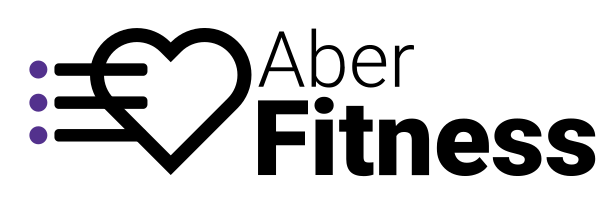
\includegraphics[width=0.5\textwidth]{Images/aberfitness.png}
\end{center}

\par
\textit{Aber Fitness} is a web application developed using Microsoft's \textit{.NET Core} and Oracle's \textit{Java Enterprise Edition} (henceforth referred to as Java EE). The project aims to provide a service which encourages fitness and promotes engagement with sporting activities amongst the users of the application, by offering functionality such as:

\begin{itemize}
	\item Graphing fitness data gathered by owners of \textit{Fitbit} devices, or through manual input.
	\item The ability to take part in challenges based on that fitness data.
	\item Providing a Sport ladder system, which has tight integration with a bespoke facility booking system.
\end{itemize}

\textit{Aber Fitness} aims to offer everything required by a sporty and active person in order to bring their sporting activities onto a digital platform and also to enhance their use of devices they already own, such as fitness tracking devices or smart watches such as the \textit{Fitbit Charge}.

\par
At launch, the system will automatically ingest activity data from \textit{Fitbit}, and be open to the addition of other health data provider services, such as Apple Watch, at a later date due to the modular nature of the data ingest system. Once normalised, this activity data will be used throughout the various microservices within \textit{Aber Fitness}, providing users with functionality such as a dashboard overview of their activity over the past month, as well as integrating tightly with the challenges microservice to add a competitive aspect to the system, with the aim of keeping users engaged with both the platform itself and keeping fit in general.

\par
\textit{Aber Fitness} will also feature a number of supporting tools, such as:

\begin{itemize}
	\item A user management system with two-factor authentication.
	\item A comprehensive audit trail of when and how their data was used and accessed, which is filterable by date.
	\item A global layout template with a dynamic sidebar, which can be adjusted by administrators. Those changes will be instantly propagated to the other microservices.
\end{itemize}

\par
\textit{Aber Fitness} is also designed to be scalable and easily deployed through the use of \textit{Docker}, by segregating related functionality into individual microservices.

\chapter{Requirements}

\section{Data Gathering and Storage}
\begin{tabular}{ |p{5cm}|l|l|p{8cm}|}
\hline
\textbf{Requirement}	&	\textbf{FR\#}	&	\textbf{Completed}	&	\textbf{Comments} \\
\hline
Management of Participants in the System			& DG-FR1	& Yes	& All sub requirements have been met. \\
\hline
Activity Data										& DG-FR2	& No	& Not all sub requirements have been met. \\
\hline
Linking a participant to a server-based data source	& DG-FR3	& Yes	& Requirement complete. \\
\hline
Obtaining data from the server-based data source	& DG-FR4	& Yes	& Requirement complete. \\
\hline
Receiving data from other devices					& DG-FR5	& Yes	& Requirement complete. \\
\hline
Receiving manual input of data						& DG-FR6	& Yes	& Requirement complete. \\
\hline
Data to retrieve 									& DG-FR7	& Yes	& Additional Requirement - All step data should be collected for the system. This will include "workout" sessions. \\
\hline
Removing data for a participant						& DG-FR8	& No	& TODO: May need changing. Not all sub requirements have been met. \\
\hline
Administrator access to data						& DG-FR9	& No	& Not all sub requirements have been met. \\
\hline
User group relationship								& DG-FR10	& Yes	& Additional Requirement - A user can exist on the system without being part of  a group. If a user joins a group they can only be associated with that one group. \\
\hline
Activity data management							& DG-FR11	& Yes	& Additional Requirement - An interface should be provided for the administrator to map FitBit activities to the activities created for the system. \\
\hline
\end{tabular}

\section{User Management}
\begin{tabular}{ |p{5cm}|l|l|p{8cm}|}
\hline
\textbf{Requirement}	&	\textbf{FR\#}	&	\textbf{Completed}	&	\textbf{Comments} \\
\hline
Authentication and authorisation 					& UM-FR1 	& Yes 		& Requirement Complete. \\
\hline
Local User Accounts 								& UM-FR2 	& Yes 		& Additional Requirement - The user accounts do not need to be Aberystwyth University integrated. Local user accounts should be used. \\
\hline
User Characteristics								& UM-FR3	& Yes		& Requirement specified in document but not given a functional requirement number. There will be three different types of users: member, coordinator and administrator. \\

\hline
\end{tabular}



\section{Health Dashboard}
\begin{tabular}{ |p{5cm}|l|l|p{8cm}|}
\hline
\textbf{Requirement}	&	\textbf{FR\#}	&	\textbf{Completed}	&	\textbf{Comments} \\
\hline
Review data for a member 							& HD-FR1 	& Yes 		& Requirement complete. \\
\hline
Set goals and view progress. 						& HD-FR2 	& Yes		& Requirement complete. \\

\hline
\end{tabular}


\section{Challenges}
\begin{tabular}{ |p{5cm}|l|l|p{8cm}|}
\hline
\textbf{Requirement}	&	\textbf{FR\#}	&	\textbf{Completed}	&	\textbf{Comments} \\
\hline
Create a challenge 									& C-FR1 	& Yes 		& Requirement Complete. \\
\hline
Join a challenge 									& C-FR2 	& Yes  		& Requirement Complete. \\
\hline
Activity during a challenge							& C-FR3 	& Yes 		& Requirement Complete. \\
\hline
Closing the challenge								& C-FR4		& Yes 		& Requirement Complete. \\
\hline
Types of challenges 								& C-FR5 	& Yes		& Additional requirement - There should be two types of challenge. "Personal goals" which will be individual challenges and "Group challenges" which allows members to join challenges for their group. \\

\hline
\end{tabular}


\section{Booking System}
\begin{tabular}{ |p{5cm}|l|l|p{8cm}|}
\hline
\textbf{Requirement}	&	\textbf{FR\#}	&	\textbf{Completed}	&	\textbf{Comments} \\
\hline
Facilities      									& BS-FR1	& Yes      		& Requirement complete. \\
\hline
Availability   										& BS-FR2	& Yes      		& Requirement complete. Requirement extended - an administrator block on a facility should be a single booking not multiple hourly bookings. 	\\
\hline
Booking         									& BS-FR3	& Yes      		& Requirement complete. \\
\hline
Available Times 									& BS-FR4	& Yes      		& Additional Requirement - A fixed time for bookings should be available for a facility (9am -9pm). \\

\hline
\end{tabular}

\section{Sports Ladder}
\begin{tabular}{ |p{5cm}|l|l|p{8cm}|}
\hline
\textbf{Requirement}	&	\textbf{FR\#}	&	\textbf{Completed}	&	\textbf{Comments} \\
\hline
Creating 											& SL-FR1	& Yes 		& Requirement complete. \\
\hline
Joining 											& SL-FR2	& Yes 		& Requirement complete. \\
\hline
Profile Update 										& SL-FR3	& Yes		& Requirement complete. \\
\hline
Suspension 											& SL-FR4	& Yes 		& Requirement complete. \\
\hline
Current Ladder	 									& SL-FR5	& Yes 		& Requirement complete. \\
\hline
View Member											& SL-FR6	& Yes 		& Requirement complete. \\
\hline
Challenge 											& SL-FR7	& Yes		& Requirement complete. \\
\hline
Scheduling 											& SL-FR8	& Yes 		& Requirement complete. \\
\hline
Response to a challenge 							& SL-FR9 	& Yes 		& Requirement complete. \\
\hline
Expiry 												& SL-FR10 	& Yes		& Requirement complete. \\
\hline
Result 												& SL-FR11 	& Yes 		& Requirement complete. \\
\hline
Removal 											& SL-FR12 	& Yes 		& Requirement complete. \\
\hline
Match Involvement									& SL-FR13 	& Yes 		& Additional Requirement - As a member can only be involved in one match at a time. \\
\hline
Winning a match 									& SL-FR14 	& Yes 		& Additional Requirement - If the loser of a match is in a high position on the ladder than the loser, their position should swap with the loser on the ladder. \\

\hline
\end{tabular}

\section{Engagement}
\begin{tabular}{ |p{5cm}|l|l|p{8cm}|}
\hline
\textbf{Requirement}	&	\textbf{FR\#}	&	\textbf{Completed}	&	\textbf{Comments} \\
\hline
Current Rankings 									& E-FR1		& Yes	& Requirement complete. \\
\hline
Individual Progress									& E-FR2		& Yes	& Requirement complete. \\
\hline
Weekly Updates 										& E-FR3		& Yes	& Requirement complete. \\
\hline
Missing Reading Updates 							& E-FR4		& Yes	& Requirement complete. \\

\hline
\end{tabular}


\section{External Interface}
\begin{tabular}{ |p{5cm}|l|l|p{8cm}|}
\hline
\textbf{Requirement}	&	\textbf{FR\#}	&	\textbf{Completed}	&	\textbf{Comments} \\
\hline
Appearance & EIR1 & Yes. & Requirement Complete. \\
\hline
Internationalised Interface & EIR2 & No. & Requirement not complete. \\
\hline
Handling UI - Proxy & EIR3 & Yes. & Additional Requirement - Services should generate their own UI, the UI goes back to the client via a proxy. \\
\hline
\end{tabular}
\chapter{Development Methodolgy}

\textcolor{red}{\textbf{TODO: Possibly restructure this, it\'s a start for now. Not 100\% sure what Neil\'s looking for here.}}

Upon starting the project, we met as a group and decided on a standard style of development which would work best between all of us. After some discussion, we concluded that a \textit{Scrumban}\cite{scrumban} style of development would best fit our needs. Due to the relatively short duration of the project, and our team consisting of only eight developers, we decided on adopting this rather hands off development approach which focuses on flexibility and being able to change and adapt the project plan and sprints as the project progresses. The \textit{Scrumban} methodology was also suited to the project as the two technologies we were required to use, Java EE and .NET Core, were new to all of the members of our team, making estimating sprints and velocity quite difficult. 

We began the project by breaking the project specification down into disitinct microservices, and deciding which technologies would be best suited to each service. \textbf{TODO: Link to figure below}

\begin{figure}[H]
    \centering
    \includegraphics[width=\textwidth]{Images/Initial_Spec_Chart.jpg}
    \caption{An initial design diagram which was used to help break down the project into smaller microservices and gain a rough understanding how each microservice could interact}
\end{figure}

Once the individual microservices had been decided upon, we set out on allocating each microservice to two members of the team and assinging each service a priority ranking between 1 and 3, depending on how the services depended on one another. Services marked with a priority of 1 were core parts of the \textit{AberFitness} infrastructure on which many other parts of the system relied on their APIs in order to function correctly, such as the \textit{Health Data Repository} microservice.  \textbf{TODO: Link to figure below}

\begin{figure}[H]
    \centering
    \includegraphics[width=\textwidth]{Images/Numbering_Microservices.jpg}
    \caption{Initial plan for ordering microservices in terms of priority and allocating them to members of the team for development}
\end{figure}
\chapter{Design}

\section{System Overview}
The \textit{Aber Fitness} system is broken down into a number of microservices in order to aid portability, scalability and promotes a more maintainable codebase. After reviewing the initial project specification, the following microservices were created:

\begin{itemize}

	\item \textbf{Booking \& Facilities} - The \textit{Aber Fitness} offers functionality for users to be able to schedule bookings at sports venues, such as swimming pools and squash courts. This microservice is called used by the \textit{Ladders} service to create bookings for competitions.

	\item \textbf{Challenges} - The system offers the ability to give users activity challenges, for example completing a number of steps in a specific timeframe. These challenges can also be 'group' challenges, where a number of users can compete against each another to achieve goals such as furthest distance walked in a week, etc.

	\item \textbf{Communications} - This microservice provides an API for other services to send email notifications to users. It does not present any form of web UI, and users do not directly interact with it. This system could also be easily expanded to send out text messages, push alerts, etc. depending on future requirements.

	\item \textbf{Fitbit Ingest Service} - At launch, the \textit{Aber Fitness} platform allows a user to link their \textit{Fitbit} accounts to the system in order to import their activity data. The service periodically polls the Fitbit API for new data on the users' behalf, then stores this into the \textit{Health Data Repository}.
	
	\par With the possibility of adding future platform support the "ingest service" concept was created. This would allow us to support services such as Apple's \textit{HealthKit} and other fitness tech providers. 
	This architectural design means that activity data can be normalised by a number of "ingest services" before being passed through to the \textit{Health Data Repository} service for storage. 

	\item \textbf{Gatekeeper} - \textit{Gatekeeper} is \textit{Aber Fitness}'s OpenID Provider, and handles all authentication within the system. User credentials and account metadata is stored within \textit{Gatekeeper}\textit{Gatekeeper} uses the OAuth 2.0 flow and is responsible for providing a single sign-on service for all of the various microservices. Microservices also contact \textit{Gatekeeper} to obtain and verify tokens when calling internal APIs.

	\item \textbf{GLaDOS} - \textit{GLaDOS} is the centralised auditing mechanism for \textit{Aber Fitness}. It presents a REST API which is used to store audit data; such as when a user's data was accessed, modified, or deleted. \textit{GLaDOS} also provides a Status page which displays the availability of all the other microservices.

	\item \textbf{Health Dashboard} - \textit{Health Dashboard} is the first interface users will encounter after logging in, or navigating to \textit{Aber Fitness}.  It provides the user with an overview of their recent activity as well as providing updates on any challenges or ladder competitions the user may be involved in.

	\item \textbf{Health Data Repository} - The \textit{Health Data Repository} service is responsible for providing an API for accessing and storing activity data. It receives normalised activity data from the Ingest Services, and provides multiple API endpoints for other microservices to access user activity data. 

	\item \textbf{Ladders} - \textit{Ladders} is responsible for organising and managing ladder style competitions among users of the system. Users can compete in sporting championships for a variety of competitive sports such as tennis, running or cycling etc. The \textit{Ladders} service also automatically books venues for upcoming competitive events, which is managed by the \textit{Booking Facilities} microservice.

	\item \textbf{User Groups} - \textit{Challenges} can also be turned into a competition amongst users of a group. For example, a group may consist of a few friends or an entire office department. Users within a group compete to complete goals, such as who can achieve the most steps in a single day. The \textit{User Groups} service is responsible for managing users into groups, and allowing users to leave and join other groups.

\end{itemize}
\chapter{Implementation}

\section{Deployment}

\section{Java EE}
    \subsection{Common Components}
        \subsubsection{Handling Dependencies and Static Analysis}
        \par
        At the start of the project the JavaEE development teams agreed to use \textit{Maven}\cite{Maven} to handle their dependencies. This allows the entire build process to be ran at the commandline rather than within the IDE, which is essential for \textit{TravisCI} integration.

        \par
        Maven uses an XML file called \textit{POM.xml} to define the dependency names, versions and additional options. These are fetched from Maven Central and cached locally for future builds. To add a new dependency a developer simply visits the hosting website and copies the XML provided alongside each package. Additionally developers can use the \textit{Scope} option which instructs the packaging plugin the associated \textit{JAR} files are provided by the Payara runtime.
        
        \par
        \textit{IntelliJ} natively supports reading from Maven's \textit{POM.xml} file, which defines the list of dependencies and compilation steps. Maven also contains a plugin which allows developers to package the built files into a web archive (WAR). This did have some caveats however; running 
        `\textit{mvn war:war}' would result packaging artefacts from the previous compilation, without compiling the current application. This could lead to confusion as new changes would no be reflected without `\textit{mvn compile war:war}'.

        \par
        Whilst working locally developers could still rely on IntelliJ's built in mechanism for packaging and deploying to a local Payara instance. This allowed for rapid development feedback and iteration without the overhead imposed by Maven.

        \subsubsection{Creating Docker Images}
        \par
        By utilising the ability to run the entire build process on the command-line with Maven we were able to quickly add Travis CI integration. This would clean compile the entire application, run the full \textit{JUnit} test suite and lastly package a WAR file.

        \par
        Initially we used \textit{CheckStyle} to also enforce coding style conventions. However the rules were over-specified. Additionally, unlike other formatting tools there was no option to emit a patch-file which allows developers to automatically fix-up many errors such as incorrect white space or formatting.

        \par
        The Java teams migrated to the \textit{PMD}\cite{PMD} static analysis tool: this warns about unused fields and variables, unsafe constructs,and dangerous coding patterns.
        The Maven test target was modified to run the \textit{PMD}\cite{PMD} static analysis tool before any unit tests. If any violations were detected the build would immediately stop, ensuring all modifications were inspected.

        \par
        The groups proceeded to add a \textit{Dockerfile} to build a docker image for later deployment. Payara provide multiple images on \textit{DockerHub}\cite{DockerHub_Payara}, which range from the full server to an embedded instance.

        \par
        Initially we copied the local web archive, which was built on Travis, into the full Payara deployment folder. This allowed us to use the web administration console to resolve various deployment issues without having to dig through log files. After moving changing the default source code layout, which resolved \textit{resources} not being included in the final archive, we successfully deployed GLaDOS to the full instance.

        \par
        However we could not get Fitbit Ingest to successfully deploy, they had already started implementing the OAuth flow which is required by both the Fitbit API and our own internal API. The internal SSL implementation had changed with JDK update 191, which prevented the \textit{CDI} layer from initialising the associated beans.

        \par
        As the bundled JDK version is controlled by Payara in the base image we proceeded to look for an alternative solution. We decided against modifying the image to transplant a specific JDK at build time. Instead, we found that there was an open upstream issue\cite{payara_ssl_issue} that used reflection to resolve the problem internally. As this fix was not released into the latest stable release we had to switch to running pre-release images for all Java EE applications.

        \subsubsection{Migrating to Micro Image}
        \par
        The Payara Microprofile image is designed specifically to be used in Docker deployments. Whilst this does not implement the full EE, the memory usage is ten times lower at 90MB. The profile still provided the required set of services for the application so there was a significant benefit to completing this migration. However trying to deploy to the micro instance resulted in an exception being thrown whilst completing the implicit bean discovery phase. 

        \par
        The CDI 1.1 specification and above requires the server to automatically scan for injection points and pair it with matching enterprise Java beans (EJBs). This can fail with older dependencies, so we initially suspected one of the dependencies did not correctly use the \textit{beans.xml} annotation to turn this off.
        \newline
        Switching off bean discovery and manually annotating them allowed the ingest service to correctly deploy. However bean discovery is required for Facelets 4.0 and an exception will be thrown if it is not enabled. A new project was created with all but the essential dependencies removed, and we discovered the exception was still thrown which only added to the confusion. 
        
        \par
        By looking at the package namespaces associated with the injection points and running `mvn dependency:tree' we could see that `\textit{org.sonatype.guice}' was the culprit. Walking up the tree we discovered that the WAR plugin was being included in our packaged dependencies. At deployment the microprofile server tried to start a Maven instance and failed, thus removing this dependency correctly allowed the application to start. The development teams realised that the plugin was included in our installed copies so we could still continue to use it.

        \label{JTA_Targets}
        \subsubsection{Setting up JTA Targets}
        Both services started off by instantiating the single JDBC connection through the driver manager as required. This had some caveats however: Firstly, the JDBC driver had to be distributed and managed within the web archive. Secondly, there was no form of connection pooling to allow for scaling at the persistence layer.

        \par
        Traditionally a connection pool is created using the administration web GUI. However this would require a developer set up the pool each time continuous deployment finished on a full instance. The microprofile we had just switched to did not provide a web GUI at all.

        \par
        Glassfish allows a web application to specify resources found on the server using `glassfish-resources.xml'. This XML file can also use system environment variables allowing us to protect and specify database credentials on the deployment targets. The examples found online primarily pertained to a \textit{MySQL} deployment, so multiple iterations of testing and deployment were required to get the pool working successfully. This switch allows an application to detect and create connection pools at deployment, allowing the images to rapidly redeploy facing another database instance.

    \subsection{Fitbit Ingest Service}
        \subsubsection{To Do}

    \subsection{GLaDOS}
        \subsubsection{REST API}
        \par
        The primary role of GLaDOS is to store audit data so that users can view how their data was viewed and modified. Whilst there are native implementations, such as the Java Messaging Service, these require the calls be proxied into a local JVM instance to handle the transport component. We chose to serialise into JSON and use REST as the transport mechanism as all applications had native support for this set up.

        \par
        \textit{JAX-RS} is an API specification for JSON parsing in Java, additionally Payara provides \textit{Jersey} as the implementation of this API at runtime. This avoided us having to package additional dependencies into the web archive. This also allows us to build standard response pages based on the error code internally generated, avoiding having to develop error views.        

        \subsubsection{Unit Testing and Mocks}
        \par
        A new class abstracting the database layer allowed us to avoid writing entity handling at this. We instead focused on writing unit tests which verified the various endpoints correctly serialised or de-serialised data. \textit{Mockito}\cite{Mockito} allows developers to inject mock objects by specifying the class which the test fixture is using.

        \par
        We could not use dependency injection within the endpoint implementation, as the instantiation point is internal to the framework. This doesn't prevent us from using mocks as Mockito allows a developer to inject them through the reflection methods built into the library. A database call such as `\textit{db.getEntry(id)}' could be tested to see which status codes would be sent and verify the data,if any, was serialised correctly.

        \subsubsection{Integration Testing with Arquillian}
        \textit{Arquillian}\cite{Arquillian} allows developers to specify the classes to archive and deploy within the text fixture. Payara also provides an embedded Arquillian test container which can be ran at test time to exercise sections of a full system. This would allow us to write integration tests for an end-to-end operations, such as POSTing data to an endpoint and ensuring it is written to the persistence layer.

        \par
        There was extensive documentation on the methods required to pack an archive, but limited examples on handling Maven dependencies. As the embedded instance provides no runtime methods we were having problems getting the container to correctly run. Developers could specify the full class paths for their dependencies to ensure the were packaged, but this was extremely verbose and fragile.

        \par
        We looked into using the Maven dependency resolver, which allows developers to get a list of runtime Jars and package them into the archive. However this would led to another set of problems where Maven was trying to export them into a \textit{.zip} format, then throw an exception because this was not supported.

        \par
        With no easy was to control the format that runtime dependencies were exported in, combined with a lack of documentation pertaining specifically to Maven we agreed to abandon this method of automated testing. This would give us more time for implementing other components within the deadline. We opted to rely on manual integration testing for the duration of the project instead.

        \subsubsection{Entity Management}
        This service only persists Audit Data, therefore we ultimately need to persist a single entity. Whilst many ORM solutions exists for Java, such as \textit{Hibernate}, we decided against them due to the implementation overhead that was required.

        \par
        Instead we relied on the persistence layer provided in the EE specification. Using the connection pools which were set up for both Java services (see \ref{JTA_Targets}), we could specify which JTA the injected entity manager should use.

        \par
        The table schema is managed through annotations on an entity class. This also allows the implementation provided by Payara, \textit{EclipseLink}, to create the tables required at deployment time. As the framework relies on the field types to determine which underlying storage to use there is a hidden pitfall. If the type does not have a native serialisation Java will try to persist this using binary data.

        \par
        Instants are used to specify timestamps on logs, these are cross compatible as they use \textit{ISO 8601}\cite{ISO_8601}, a string specifier for absolute time points. This format allows both .NET Core and Java application to send timestamps in the following format \textit{2018-11-28T12:04:14Z}. However as this type was added in JDK 8 there is no native storage conversion built into the entity framework.

        \par
        Two adaptors were written based on the \textit{AttributeConverter} interface. These provide methods for marshalling and un-marshalling Instants into String objects, which the entity manager can easily store. Annotating the field installed the converting class and correctly updated the schema. This also has the added benefit of making the stored timestamps human readable within the database, which extremely helpful for debugging.

        \subsubsection{Developing Facelets}
        \par
        GLaDOS also provides a page that allows a user to retrieve audit data associated with their account. Administrators can look up any users audit data by user their unique ID too. In addition there is a status page which allows anyone to view the status of all other micro-services without logging in.

        \par
        The front-end of GLaDOS use facelets to implement the MVC pattern. A backing bean for the user data uses named queries from the persistence layer to retrieve data into a list of entity objects. We switched to using \textit{PrimeFaces}\cite{Primefaces}, which is a fork of the now deprecated \textit{RichFaces}. This allows us to use components such as \textit{DataTables} which dynamically generate tables based on the number of entries returned.

        \par
        The Fitbit Ingest Service had completed OAuth implementation for connecting to internal and external APIs. This was ported across to GLaDOS and further modified. As the ingest service has no front-end they don't need to persist \textit{JSON Web Tokens (JWTs)}. Additional methods were written specifically for this microservice. These include using the HTTP session handling built into the web framework to persist the token on the server. Another helper class was written which validates the stored JWT as the user navigates through protected pages, or POSTs any requests.

        \par
        Service statuses were implemented using a singleton Java bean which is instantiated at deployment. Using the scheduling capability provided for EJBs we poll all services every 20 seconds in a seperate thread. All services implement an endpoint at \textit{/api/status} that returns a 200 or 204. This is stored until the page is retrieved where the backing bean, acting as a presenter forward the results on.

        \par
        As the application stack uses an \textit{nginx} instance to reverse proxy queries the URLs must take this into account when they are generated within the facelet. .NET Core makes this trivial by calling `\textit{App.UsePathBase(URL)}' at start up, however Java applications rely on the context root. This was interfering with the URL rewriting that Nginx performs resulting in the service using the 
        `\textit{/glados/glados/}' base path.

        \par
        Initially we used an environment variable to manually generate links between the pages of the service and set the context root to 
        `\textit{/}'. However, this quickly proved to be untenable when using forms, as POST requests were being sent to 
        `\textit{/destination}' 
        rather than 
        `\textit{/glados/destination}'. Ultimately to work around this an exception was added to Nginx configuration to avoid re-writing any URLs for GLaDOS, and instead rely on the service to correctly address all requests. This allowed us to switch back to generating addresses based on the \textit{outcome} tag and use forms on the service.



\section{.NET Core}
    \subsection{}{Common Components}
some blurb about .net core here

    \subsection{Booking Facilities}

    \subsection{Challenges}

    \subsection{Communications}

    \subsection{Gatekeeper}

    \subsection{Health Data Repository}

    \subsection{Health Dashboard}

    \subsection{Ladders}

    \subsection{User Groups}

\chapter{Testing}
\par
One of the core tenets of continuous deployment is the reliance on a mix of automated and manual testing to ensure a system is functioning correctly. The applicable subset of these tests were run before each change specified in a pull request was accepted. The full suite is run as part of the release process, allowing developers to deploy the application to production with confidence.

- XUnit - recommended and widely used, Moq
- Moq - Gatekeeper
- JUnit
- Mockito - GLaDOS / Ingest (to fix)


\section{Integration Testing}
\par
Most of the micro-services provide internal APIs, which are not designed for external usage. To protect these endpoints the OAuth 2.0 flow was used to authorize application interactions with client credentials. Whilst unit testing ensures each API correctly responds according to its documented behaviour, it does not exercise all components that partake in an interaction.

\par
As REST endpoints were used as the primary message exchange method we could send and request JSON payloads to ensure the system under test behaved as expected. Multiple third party solutions were used for testing APIs, \textit{Postman}\cite{Postman} was one instance that was widely used by the development team. 
This can handle the OAuth flow 

\par
Developers used these tools to ensure that malformed requests or interaction with no authorization token were correctly handled. Additionally they can handle the OAuth flow on a developers behalf, this was extremely useful when debugging interactions between applications and resolving digressions from the API specifications.


\section{System Testing}
\par
Aber Fitness is deployed onto two separate docker hosts that represent staging and production. Developers trigger a deployment from the latest development images in Slack then manually test the system in a deployed state. This also allows us to detect deployment specific problems, which are un-testable without a complete system.

\par
One example of an issue caught by manual system testing was a controller which was not asynchronous. Unit tests would not exercise the instance in parallel, so this was not noticed through unit testing. When API calls were made to the deployed application a HTTP 502 was thrown. The controller was blocked on the original call and could not respond to the next call.


\section{Static Analysis}
\subsection{PMD}
\par
Initially, Java used \textit{CheckStyle} to also enforce coding style conventions. However, the rules were far too strict to be beneficial or practical and, unlike other formatting tools, there was no option to emit a patch-file which allows developers to automatically fix-up many errors such as incorrect white space or formatting.

\par
The Java teams later migrated to the \textit{PMD}\cite{PMD} static analysis tool: this warns about unused fields and variables, unsafe constructs, and dangerous coding patterns.
The Maven test target was modified to run the PMD static analysis tool before any unit tests. If any violations were detected the build would immediately stop, ensuring all modifications were inspected.

\section{Acceptance Testing}
\par
During our first meeting, the project's functional requirements were broken down into a number of spreadsheets, each based on the service which would implement them. The client was then contacted to clarify any requirements which were ambiguous to the group. Acceptance tests for each micro-service were created in a spreadsheet based on these original and revised requirements.

\par
Acceptance tests are completed manually by completing the steps defined by the document. Each test is marked as either pass or fail based on the criteria set out in the document, allowing the individual microservices, and by extension the entire project, to be assessed on its fitness for purpose.

\par
A fresh deployment of the system was performed shortly after a code freeze and the full suite of acceptance tests were completed. This round of testing highlighted 23 instances where the implementation deviated from the client's requirements.

\par
Bugs were assessed on a case-by-case basis, taking account of the impact. Fixes which had a low potential for regression and addressed high impact problems were implemented and merged after the code freeze. This process resolved 11 of those implementation issues, resulting in almost half of the failed acceptance tests becoming passes in the space of a few hours, and with no additional issues appearing as side-effects. This shows that internal acceptance testing was a highly valuable process that resulted in a noticeable improvement in the final product.

\chapter{Status}

\section{Overall System}
    Overall, the vast majority of the client's requirements have been developed and implemented successfully. Any outstanding bugs or features not implemented which are specific to individual microservices are noted in the following subsections.

Four acceptance tests were defined for the system as a whole, with the acceptance test table available in Appendix 2, Section 0.2.1. Of these four tests, only one failed. The failed test required that the system support localisation. It was decided amongst the group that, due to time restraints, localisation would be left until later on in the project when it could be re-evaluated whether or not there was time to implement the feature. While localisation was investigated as part of the spike work, once the system was implemented there was not enough time to modify the existing views and prepare them for integration with a localisation system.

\section{Booking Facilities}
    \subsubsection{MVC Architecture}
\par
The \textit{Booking \& Facilities} microservice was created to allow users to make, view, modify, and remove their bookings for sport activities at their local sports venue. As bookings are created directly from the microservice or the \textit{Sports Ladder}, it made sense for the \textit{Booking \& Facilities} system to have its own persistence layer that stored data on bookings, venues, sports and facilities. 
\par
Thus \textit{FacilitiesController}, \textit{VenuesController}, \textit{SportsController},  and \textit{BookingsController} were created, each performing basic CRUD operations on their respective areas with a view and API for each. A simple status API was also written to give the microservice's current internal status. 
\par 
The system design went through several iterations before a design was finalised. One particular issue stemmed from uncertainty regarding how facilities and sports would link together due to ambiguity in the client's requirements. Following clarification from the client, the model was reworked so that a facility could only be associated with a single sport. The final implementation allows multiple facilities with the same name to exist within a venue, but a facility-sport combination must be unique within that venue.
\par 
As a booking takes one specific facility, it was logical to assign a venue and a sport to a facility, and for the latter two simply containing an ID and name field. Normalising the data resulted in more complexity in the controllers, but simplified the persisted data.
\par
Another aspect of the model which was redesigned was a booking requiring an end date, alongside the pre-existing start date. This was done to accommodate the concept of a facility block; allowing an administrator to prevent users booking a facility for a period of time. This would also remove any previously created bookings during the block. To implement this a boolean was added to the \textit{Booking} model specifying that the booking exists as a block. When booking normal slots a user still provides a start date without an end date, as bookings are designed to last for exactly an hour.
\subsubsection{API Endpoints}
\par 
Several API calls to \textit{Booking \& Facilities} are made from the microservice itself to get the sports, times, and update a booking's details. The only other microservice which interacts with the \textit{Booking \& Facilities} system is the \textit{Sports Ladder}. This relies on the ability to view all booking data (sports, venues, facilities and bookings/blocks), as well as create and delete bookings within the ladder. The API accommodates for this, with some slight adjustments made during the implementation of the \textit{Sports Ladder}. 
\subsubsection{User Interface Style}
\par 
Users are also able to directly create and modify their own bookings. The requirements made it necessary for an administrator to delete, modify and see all user bookings. Due to the basic nature of how this data was handled there were no complex visualisations; all data is displayed in tabular form and new entries are created and updated with simple forms.


\section{Challenges}
    \begin{figure}[H]
    \centering
    \includegraphics[width=\textwidth]{Images/service_challenges.png}
    \caption{A screenshot demonstrating the Dashboard service integrating Challenges data, and displaying the user progress on challenges that they're a part of}
\end{figure}

\section{Fitbit Ingest Service}
    % TODO Who knows what's going on here? Not me.

Please see acceptance test table in Appendix 2, Section 0.2.4.

\section{Gatekeeper}
    \begin{figure}[H]
    \centering
    \includegraphics[width=\textwidth]{Images/service_landing_page.png}
    \caption{Gatekeeper is responsible for serving up the landing page, which features a user log in form and the ability for users to register to join Aber Fitness}
\end{figure}

\section{GLaDOS}
    \begin{longtable}{ |l|p{3cm}|l|p{5cm}|p{5cm}|l|p{6.5cm}|}
\hline
\textbf{FR\#}	&	\textbf{Requirement} & \textbf{AT\#}	&	\textbf{Description} & \textbf{Test} & \textbf{Pass/Fail} &	\textbf{Comments} \\
\hline
\endhead

DG-FR9-1 & Users should be able to access their own audit data & GL-AT-11 & When the user visits the Audit data page, they should be able to view their data associated with their account & Create a new account and perform an action which edits data. E.g. adding a manual entry. Go to the audit log pages and ensure it appears in a human readable form. & Pass & Data is present, but the format of the "content" provided by each service is inconsistent.  The page could automatically load data for the past X days rather than the default value of the 'From' input being the current time. \\ \hline
DG-FR9-1 & Users should not be able to view other peoples' access data & GL-AT-12 & The user ID field should be greyed out and not editable. This should be server side validated & Ensure text in box cannot be modified. Edit the text using debugging console in browser, ensure the page returns with the original unmodified ID & Pass & The input for User ID could be hidden for users who aren't able to edit the value.  \\ \hline
DG-FR9-2 & Administrators should be able to access audit data for any user in the system & GL-AT-21 & An administrator should be able to view their own Audit data. & Login as an administrator and perform and action which edits data, E.g. adding a manual entry. Go to the audit log pages and ensure it appears in a human readable form. & Pass & See comments for GL-AT-11  \\ \hline
DG-FR9-2 & Administrators should be able to access audit data for any user in the system & GL-AT-22 & An administrator should be able to view other users Audit data. & Login to the user account and copy the unique user ID. Log back in as the administrator and change the ID in the text box to this. Ensure that the audit logs returned are for the queried user. & Pass & It would be better if a human-readable identifier such as an email address could be entered, rather an than a UUID.  There's no intuitive way for an administrator to get the UUID of a user other than going to the user management pages, and viewing the UUID for that user in the browser URL. \\ \hline
N/A & N/A & GL-AT-31 & A user who is not logged in should be able to view the service status & Open the service status as both a logged in and logged out user. These should correctly reflect the microservices running. & Pass & Upon system start up, the page shows the GLaDOS service as being down, despite it clearly being up by virtue of being able to display the status page.  There is no way for users who aren't logged in to find the status page, unless they know the direct URL to the page. \\ \hline


\end{longtable}

\section{Health Dashboard}
    \subsubsection{MVC Architecture}
\par
The Health Dashboard was included in the design of the system to allow users to visualise and add to their activity data, personal goals and group challenges. To this end, the Health Dashboard does not have a need for a persistence layer, as all of the data it processes are stored and accessed from other microservices on the system. This lead to the service being designed initially with one controller and its associated views, with model classes existing only to aid in manipulating retrieved data.

\par
Initially the service was to only have one controller, \textit{DashboardController}, but part-way through the project it was noted that splitting off the administrative functionality of the Health Dashboard to another controller could be worthwhile. Later on in the project it was decided that administrative functionality would be better placed in microservices that control the data, and so the concept was dropped. The name of the single controller was later changed to \textit{HomeController} for semantic and technical reasons associated with a repeated pattern in the URL (\textit{dockerN.aberfitness.biz/dashboard/dashboard/\{action\}}).

\subsubsection{Data Visualisation}
\par
Lorem graphsum

\subsubsection{User Interface Style and AJAX}
\par
Lorem ipsum gentelella

\subsubsection{Headless Testing and Mocking}
\par
Lorem phantom casper sit amet


\section{Health Data Repository}
    \subsubsection{Summary}
Primarily, this microservice was fairly straightforward to develop. Most of the microservice was generated through \textit{Visual Studio}'s ability to scaffold controllers once models had been defined. A few behaviours needed more thought or needed discussion with the client, and are discussed below.

\subsubsection{Mapping Activities}

One of the first and main issues that were identified was that of how the application would handle normalising data from Fitbit and potentially other activity data providers. After some investigation, it was found that the Fitbit API didn't have a consistent format in how it returned what type of activity the user had performed; for example, Fitbit could return \textit{"Skiing 5\% slope"} and \textit{"Skiing 10\% slope"}. This lack of generalisation among activity types was identified as something that would cause the platform issues should other ingest services be developed in the future. 

Many solutions were discussed for this problem, such as having the application dynamically create activities as they were imported. Ultimately it was decided that the most robust solution which provided a consistent user experience would be to create a table which maps a variety of Fitbit activity identifiers onto a single \textit{Aber Fitness} activity (Fig. \ref{fig:health_mappings}). This idea was presented to the client and was implemented shortly after.

\begin{figure}[H]
    \centering
    \includegraphics[width=0.7\textwidth]{Images/Chpt5_HealthData_Mapping.png}
    \caption{The administrative interface presented by \textit{Health Data Repository} which allows an administrator to create new mappings for activity types}
    \label{fig:health_mappings}
\end{figure}

The above interface was implemented into \textit{Aber Fitness} and provides an easily updated and flexible way for administrators to map custom external API activity identifiers onto internal activity resources. 

Ingest services are then offered an API endpoint by Health Data Repository which allows those services to retrieve the mapping table in order to determine the most appropriate Activity ID to map the data onto.

\subsubsection{Storing Step Data}
Initially, it was planned that the \textit{Fitbit Ingest Service} would be updating the \textit{Health Data Repository} with user's step counts on an hourly basis. In order to avoid an excessive quantity of activities being inserted into the database, it was decided that an activity would be created per day and updated hourly as steps came through from Fitbit. Therefore, it was required that an endpoint be available for step counts to be updated rather than inserting a new activity every hour. 

From experience with other MVC frameworks, it was assumed that .NET Core would have the ability to "Create Model, If Exists Update". This functionality is a standard part of SQL with the \lstinline{CREATE IF EXISTS UPDATE} syntax. It was surprising to find that .NET Core did not offer this functionality natively, and resulted in more code being written than was felt necessary had another framework been used. 

Ultimately this functionality was removed once it was discovered that we were unable to obtain step count data from Fitbit on an hourly basis, and therefore the additional API endpoints developed were no longer necessary. 

\section{Ladders}
    \begin{longtable}{ |l|p{3cm}|l|p{5cm}|p{5cm}|l|p{6.5cm}|}
\hline
\textbf{FR\#}	&	\textbf{Requirement} & \textbf{AT\#}	&	\textbf{Description} & \textbf{Test} & \textbf{Pass/Fail} &	\textbf{Comments} \\
\hline
\endhead

SL-FR1-1 & An administrator can create a ladder for a specified sport. & SL-AT-1 & When an administrator is logged in they should be able to create a new ladder & Login as an Administrator, go to the ladders and create one with a new name. Associate the ladder with an existing sport. Ensure the ladder creates correctly & Fail & An admin can create a ladder, but can not associate the ladder with a sport. \\ \hline
SL-FR2-1 & Members should be able to register to join the ladder & SL-AT-2 & A user should be able to join an existing ladder. & Login as a user, try to join a ladder. Check the current user has been added to the ladder once the user has been approved by the admin. & Pass & If the admin rejects the user, they will not be added. \\ \hline
SL-FR2-1 & Members should be able to register to join the ladder & SL-AT-3 & A user should not be able to join a ladder twice & Login as a user, try to join a ladder your already a member of. Check that this is not allowed. & Pass &  \\ \hline
SL-FR2-1 & Members should be able to register to join the ladder & SL-AT-4 & A user should not be able to join a ladder which has been deleted & On a separate machine login as an administrator. As the user start attempting to join the ladder, before submitting as the administrator delete the ladder. Check this is handled correctly. & Pass &  \\ \hline
SL-FR2-2 & Members should be able to give a small profile of themselves as a member of the ladder. & SL-AT-5 & A user should be able to save a profile & Join an existing ladder, attempt to save a new user profile. Ensure that the changes persist. & Pass &  \\ \hline
SL-FR2-3 & Profiles include a general indication of availability to play. & SL-AT-6 & Users should be able to add text which indicates their availability & As a member of an existing ladder open the profile and add a section on availability. Proceed to save the profile and check the changes persist. & Pass &  \\ \hline
SL-FR2-3 & Profiles include a general indication of availability to play. & SL-AT-7 & Users should be able to add text which indicates their availability & Login as two different users in different sessions. The first user should add text that states their availability. As the second user lookup the first user profile and view this text. & Pass &  \\ \hline
SL-FR2-4 & Profiles include a preferred location of play & SL-AT-8 & Users should be able to add text which indicates their preferred location of play & As a member of an existing ladder open the profile and add a section on location preferences. Proceed to save the profile and check the changes persist. & Pass &  \\ \hline
SL-FR2-4 & Profiles include a preferred location of play & SL-AT-9 & Users should be able to add text which indicates their preferred location of play & Login as two different users in different sessions. The first user should add text that states their location preference. As the second user lookup the first user profile and view this text. & Pass &  \\ \hline
SL-FR4-1 & Ladder members can suspend their participation & SL-AT-10 & A ladder member should be able to suspend participation in it & As a member of an existing ladder, go to your profile and click suspend. Ensure the change is persisted. & Pass &  \\ \hline
SL-FR4-2 & Ladder members can resume participation & SL-AT-11 & A ladder member should be able to resume after suspending at any point & As a member of a ladder with a suspended profile, attempt to un-suspend and check the changes persist. & Pass &  \\ \hline
SL-FR4-3 & Challenges are conceded whilst suspended & SL-AT-12 & Suspended ladder members should automatically conceded all games whilst suspended. & Login as two different users in different sessions. The first user should challenge the second. The first user should mark themselves as suspended and the second should win automatically. & Pass &  \\ \hline
SL-FR4-3 & Challenges are conceded whilst suspended & SL-AT-13 & Ladder members who unsuspend should no longer automatically conceded all games & Login as two different users in different sessions. The first user should mark and unmark themselves as suspended. The second user should challenge the first again. & Pass &  \\ \hline
SL-FR5-1 & A ladder member should be able to view the whole ladder & SL-AT-14 & As a member view the ladder we should see all other members & As a member of an existing ladder browse it, ensure all joined members are present. & Pass &  \\ \hline
SL-FR5-2 & A ladder member should be able to view the whole ladder & SL-AT-15 & As a member we should see all current positions and outstanding challenges & As a ladder member browse and ensure the ranking of all members is displayed. Issue a new challenge and check this appears with existing outstanding challenges. & Pass & When a member leaves the ladder, they take their rank with them. \\ \hline
SL-FR6-2 & Other member's profiles should show details on position, outstanding challenges and the results of the last 5 matches & SL-AT-16 & View another members current position in the ladder & In an existing league, view another member's profile and check that their current position is displayed correctly & Pass &  \\ \hline
SL-FR6-2 & Other member's profiles should show details on position, outstanding challenges and the results of the last 5 matches & SL-AT-17 & View another members current outstanding challenges in the ladder & In an existing league, view another member's profile and check that their current outstanding challenges is displayed correctly & Pass &  \\ \hline
SL-FR6-2 & Other member's profiles should show details on position, outstanding challenges and the results of the last 5 matches & SL-AT-18 & View another members last 5 matches in the ladder & In an existing league, view another member's profile and check that the last 5 matches is displayed correctly & Pass &  \\ \hline
SL-FR7-1 & A user should be able to challenge the 5 users who are ranked above them & SL-AT-19 & A user should be able to challenge 5 users above them & Go to a ladder with 7 users. As the lowest ranked user ensure you cannot challenge users below you. Attempt to challenge 5 users above you, conceding after each one. Check that you cannot challenge the user 6 ranks above & Pass &  \\ \hline
SL-FR7-1 & A user should be able to challenge the 5 users who are ranked above them & SL-AT-20 & A user should only be able to challenge those above them. & As a user who is second in a league check you can only challenge the top of the league. Switch to the user who is top, ensure nobody can be challenged. & Pass &  \\ \hline
SL-FR7-2 & Users who are suspended should not count as one of the 5 challengeable users & SL-AT-21 & A user can challenge 5 users above them regardless of suspension & Go to a ladder with 7 users, suspend one of the mid ranked users. Log in as the lowest ranked user, check that the 5 users above can be challenged as if the suspended user is not present. & Pass &  \\ \hline
SL-FR7-3 & A user can only challenge one person at a time & SL-AT-22 & Attempt to challenge multiple users at once & Once one challenge is issued a user should not be able to challenge another until they conceded or win. conceded and attempt to send another challenge which should be allowed. & Pass & The challenge label is shown but clicking on it will not challenge. \\ \hline
SL-FR7-4 & Challenges cannot be issued to users who are participating in a challenge of any kind & SL-AT-23 & Users who are already challenged cannot be challenged by someone else & Challenge another user, using a third account check that the challenged user cannot be challenged . & Pass & The challenge label is shown but clicking on it will not challenge. \\ \hline
SL-FR7-4 & Challenges cannot be issued to users who are participating in a challenge of any kind & SL-AT-24 & Users who issued a challenge cannot be challenged by someone else & Challenge another user, using a third account check that the issuing user cannot be challenged. & Pass &  \\ \hline
SL-FR8-1 & When a challenge is issued the challenger should be able to select a time and venue based on availability from the booking system & SL-AT-25 & Creating Booking & When a challenge is created, a booking should be made in the booking facilities service. & Pass &  \\ \hline
SL-FR8-1 & When a challenge is issued the challenger should be able to select a time and venue based on availability from the booking system & SL-AT-26 & Removing Booking & When a match is conceded, the original booking made should be removed. & Pass &  \\ \hline
SL-FR8-1 & When a challenge is issued the challenger should be able to select a time and venue based on availability from the booking system & SL-AT-27 & Removing Booking & When a match is reorganised, the original booking should be removed. & Pass &  \\ \hline
SL-FR8-1 & When a challenge is issued the challenger should be able to select a time and venue based on availability from the booking system & SL-AT-28 & Creating Booking & When a match is reorganised, a new booking should be made. & Pass &  \\ \hline
SL-FR8-1 & When a challenge is issued the challenger should be able to select a time and venue based on availability from the booking system & SL-AT-29 & A user issuing a challenge should be able to pick a venue and time & Challenge another user, select a venue and time to book. & Pass &  \\ \hline
SL-FR8-1 & When a challenge is issued the challenger should be able to select a time and venue based on availability from the booking system & SL-AT-30 & A user issuing a challenge should not be able to book a previously booked venue & Challenge another user, select a venue and time to book. & Pass &  \\ \hline
SL-FR8-2 & When a challenge is issued the booking system should automatically book the requested venue & SL-AT-31 & A challenge should automatically book venue & Challenge another user, select a venue and time to book. Check that the slot has correctly been booked out. & Pass &  \\ \hline
SL-FR8-3 & Communications containing the full match details should be send out to participating users & SL-AT-32 & Check an email is sent when the match is confirmed & Challenge another user and accept the match, both user emails should receive an email with the match details & Pass & On re-organising a challenge, an email is not sent with the updated date/time \\ \hline
SL-FR9-1 & Challenges users should be able to accept, concede or request a change & SL-AT-33 & Check a challenged user can perform one of the specified actions when challenged & Challenge a user choose to accept & Pass &  \\ \hline
SL-FR9-1 & Challenges users should be able to accept, concede or request a change & SL-AT-34 & Check a challenged user can perform one of the specified actions when challenged & Challenge a user choose to concede & Pass &  \\ \hline
SL-FR9-1 & Challenges users should be able to accept, concede or request a change & SL-AT-35 & Check a challenged user can perform one of the specified actions when challenged & Challenge a user, choose to re-organise the challenge on the challenged users account. & Pass &  \\ \hline
SL-FR12-1 & An administrator can remove a member of a ladder at any time & SL-AT-36 & Remove an existing member as administrator & Login as an administrator, remove a user and ensure that it is persisted. & Pass &  \\ \hline
SL-FR12-2 & An administrator can remove a member of a ladder at any time & SL-AT-37 & A removed user should concede any challenges they have associated & Be challenged by another member of the leauge, switch to an administrator. Check that removing the user correctly concedes any pending challenges against them. & Fail & If any user removes themselves from a ladder, and then rejoins, they can no longer edit the ladder. \\ \hline
SL-FR12-3 & An administrator can remove a member of a ladder at any time & SL-AT-38 & A removed user who has issued any challenges should have them withdrawn & Challenge another member of the ladder, as the administrator remove the user and check that their challenge is withdrawn against the existing user. & Fail & If any user removes themselves from a ladder, and then rejoins, they can no longer edit the ladder. \\ \hline



\end{longtable}

\section{Layout Service}
    \begin{figure}[H]
    \centering
    \includegraphics[width=\textwidth]{Images/service_cms.png}
    \caption{The administrative interface offered by the Layout service to enable administrators to customize the links displayed on the sidebar of each .NET Core microservice}
\end{figure}

\section{User Groups}
    \begin{figure}[H]
    \centering
    \includegraphics[width=\textwidth]{Images/service_groups.png}
    \caption{The User Groups service allows an administrator or co-ordinator to add, edit or delete groups, and allows users to join or leave groups}
\end{figure}
\chapter{Evaluation}

\section{Development Methodology}

  \subsection{Evaluation}
  \par
  The group met for weekly meetings at the start of the project to define a top-level system design on a whiteboard. These sessions were initially productive, as work was distributed to subteams and a unified approach for the various microservices was decided. As the project went on, the usefulness of these meetings was questioned. Attempts to design by committee would rapidly devolve into either a few interested parties talking about a single service, or every developer inputting an opinion on simple decisions.

  \par
  A vote unanimously agreed to change the group meeting into a session where every developer would work on implementation in the same room instead. This refocused teams onto their own design, whilst allowing an individual to still propose system-level questions or ideas in person. Productivity also rapidly increased as knowledge of common problems and solutions were shared amongst the group.

  \par
  Throughout the project there have been instances where the requirements were not clear. Reasons ranged from multiple interpretations, noun and verb conflation, and insufficient detail. Slack was used as a communication mechanism with the client, which allowed the client to choose an appropriate time to respond to requests, which could be sent at any time, while also enabling real time discussion. These communications taking place over recorded medium meant that an answer could be easily converted into an additional requirement later.

  \par
  As the project progressed, Scrumban-related processes were skipped increasingly. Project boards weren't being updated or tracked and work was completed without an associated issue or project board entry. As there were eight members of the group, it became increasingly difficult to track the work that individual teams had remaining. Ultimately this lead to deadlines being missed, as teams had to estimate their work left to complete rather than having a metric to rely on.

  \par
  As the scope of each unit's work was not defined, branches would often contain multiple features and fixes. Pull requests would often alternate between being too large to sensibly review, or a single fix spread across several pull requests. Additionally, developers would typically review within a subteam, instead of examining other services' code. This lead to code reviews being approved without the approver properly reviewing the change. This culminated into several simple bugs and version control issues, which would likely have been spotted, such as incorrect equality comparisons being merged into the codebase.

  \subsection{Future Improvements}
  Many of the aforementioned issues would have been resolved by nominating a designated team leader. This person would ensure the work being completed has an accompanying issue which exists on a project board. They would also ensure that reviews are completed correctly and that different subteams are reviewing each other's code.

  \par
  Additional work meetings in the week would reduce the timespan between a difficult problem being discovered and co-developers being able to help in diagnosis and resolution. It would also create another opportunity for knowledge transfer across subteams in person.


\section{Future Improvements}

  \subsection{Localisation}
  \par
  Localisation was a system level requirement which was not completed. It was kept in mind during the start of the project, but no work was done in preparing the views for its introduction. In future projects, code reviews would be used to make sure that views are prepared for localisation before the barrier-to-entry becomes too high.

  \subsection{Access Tokens}
  There is currently no way to revoke a token using the authorization server. If a client token were leaked, a malicious party would be able use that token until expiration. Additionally, in \textit{Fitbit Ingest}, we currently cannot revoke a token on the user's behalf. Both of these limitations were noticed after a code freeze. Additional discussion of various use-cases would have highlighted this issue earlier in development, allowing them to be rectified.

  \subsection{Automated Testing}
  \par
  Additional development time writing automated integration tests would have reduced the ongoing maintenance costs associated with the system. All endpoints are currently tested manually; the time spent testing did not outweigh the time writing tests in this instance, however the cost-benefit would certainly pay off in the long term.

\section{Fitness for Purpose}
  \subsection{Design Constraints}
  \par
  Our application stack makes use of both \textit{Java EE} and \textit{.NET Core}, as per the design constraints. These languages also provide access to many frameworks and third party libraries and packages through Nuget and Maven.

  \par
  By carefully checking the licenses of all external code and finding alternatives where required, the system is completely free of proprietary software and licensing limitations. Additionally, the use of external packages for core components, such as \textit{Identity Server} for authorization, reduces the sites future maintenance overhead.

  \par
  Finally, deployable Docker images are created for each microservice to run on the destination server. This allows the system to scale the number of instances based on an individual service's load.

  \subsection{Functional Requirements}
  \par
  Based on the client's criteria, we have fulfilled the majority of the functional requirements, as seen in \ref{Requirements_chpt}. This was measured using acceptance tests, which give a rough indication of conformity to the requirements. 129 tests were performed with 12 failing, meeting 90.7\% of the requirements.



\end{thebibliography}

\end{document}
